% !TEX encoding = UTF-8 Unicode
% ------------------------------------------------------------------------------
% Este fichero es parte de la plantilla LaTeX para la realización de Proyectos
% Final de Grado, protegido bajo los términos de la licencia GFDL.
% Para más información, la licencia completa viene incluida en el
% fichero fdl-1.3.tex

% Copyright (C) 2012 SPI-FM. Universidad de Cádiz
% ------------------------------------------------------------------------------


Esta sección cubre el análisis del sistema de información a desarrollar, haciendo uso del lenguaje de modelado UML.

\section{Modelo Conceptual} \label{sec:modelo-conceptual}

El diagrama conceptual de clases UML que muestra la figura \ref{fig:modelo-conceptual} es la presentación gráfica de las clases necesarias para llegar a la solución del problema deseada, así como sus atributos, relaciones, etc. Nos basaremos en él para la posterior programación del software, donde cada clase del diagrama UML quedará representada por una clase Java. 

\vspace{15mm}

\begin{figure}
\centering
  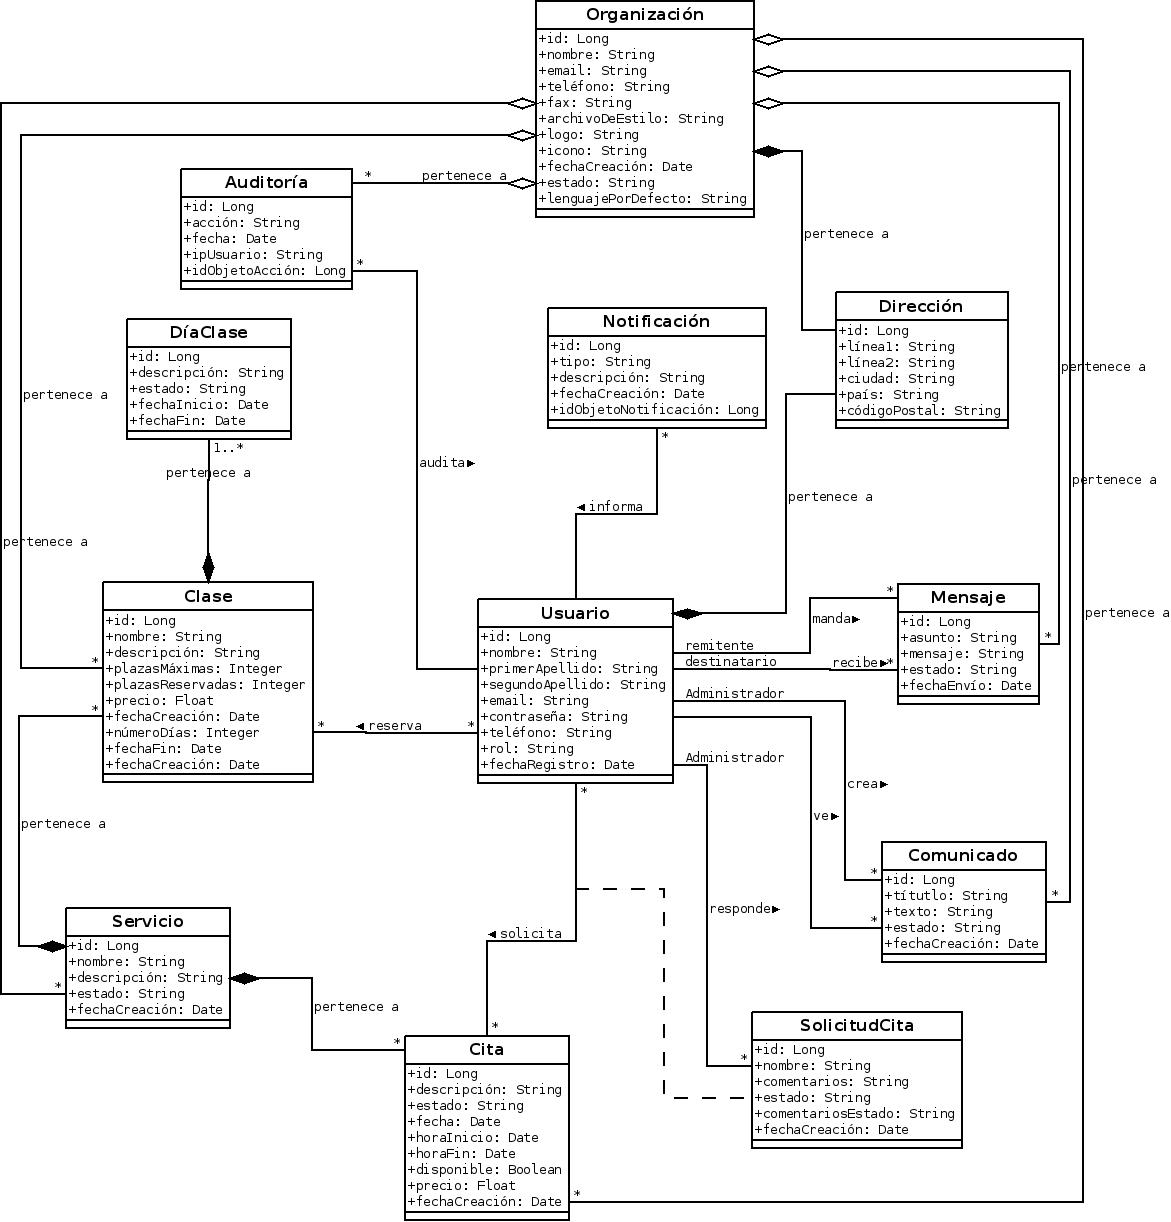
\includegraphics[scale=.35]{img/modelo-conceptual.jpeg}
  \caption{Modelo Conceptual de Clases UML}
  \label{fig:modelo-conceptual}
\end{figure}


\section{Modelo de Casos de Uso}

A continuación se describirán los principales casos de uso que se llevarán a cabo en el sistema, correspondientes a los requisitos funcionales listados anteriormente en el apartado \ref{subsec:requisitosfuncionales}. Estos casos de uso se pueden emplear como mecanismo para representar las interacciones entre los actores y el sistema:


\begin{table}[H]
  \begin{center}
    \begin{tabularx}{16.4cm}{|l|X|}
      \hline
      \textbf{UC-01} & \textbf{Seleccionar idioma}\\
      \hline
      \textbf{Descripción} & Cambiar el idioma en el que se muestra la aplicación.\\
      \hline
      \textbf{Actores} & Usuario, administrador o superadministrador.\\
      \hline
      \textbf{Precondiciones} & Ninguna.\\
      \hline
      \textbf{Postcondiciones} & El idioma de la aplicación se establecerá al que el usuario seleccione. Se establecerá este lenguaje por defecto para el usuario.\\
      \hline
      \textbf{Escenario principal} & \smallskip 1. El usuario selecciona uno de los idiomas disponibles en la lista de selección del mismo, en cualquier pantalla de la aplicación.\\
      & 2. La aplicación se mostrará en el idioma seleccionado.\\
      & 3. El idioma se establece por defecto para el resto de veces que el usuario acceda a la aplicación.\\
      & \\
      \hline
      \textbf{Escenarios alternativos} & \\
      & \\
      \hline
    \end{tabularx}
    \caption{UC-01: Seleccionar idioma}
    \label{tab:CU-idioma}
  \end{center}
\end{table}


\begin{table}[H]
  \begin{center}
    \begin{tabularx}{16.4cm}{|l|X|}
      \hline
      \textbf{UC-02} & \textbf{Registro}\\
      \hline
      \textbf{Descripción} & Registro de usuario en el sistema.\\
      \hline
      \textbf{Actores} & Usuario.\\
      \hline
      \textbf{Precondiciones} & El usuario no puede haberse registrado previamente.\\
      \hline
      \textbf{Postcondiciones} & El usuario quedará registrado en el sistema y se mostrará la página de inicio del mismo.\\
      \hline
      \textbf{Escenario principal} & \smallskip 1. El sistema muestra la página de registro con los campos correspondientes.\\
      & 2. El usuario rellena al menos los campos obligatorios y marca la casilla de aceptación de términos y condiciones. \\
      & 3. Una vez aceptado los términos y condiciones, el sistema habilita el botón de registro. \\ 
      & 4. El usuario hace click en el botón de registro.\\
      & 5. El sistema valida los datos y registra al usuario en la base de datos.\\
      & 6. El sistema realiza el login del usuario y lo redirige automáticamente a la página de inicio de la aplicación.\\
      & \\
      \hline
      \textbf{Escenarios alternativos} & \smallskip 5.a. Los datos introducidos no son válidos:\\
      & \hspace{0.3cm} 5.a.1. El sistema muestra el mensaje de error correspondiente.\\
      & \hspace{0.3cm} 5.a.2. Vuelve al paso 2.\\
      & \\
      \hline
    \end{tabularx}
    \caption{UC-02: Gestión de usuarios: Registro}
    \label{tab:CU-registro}
  \end{center}
\end{table}


\begin{table}
  \begin{center}
    \begin{tabularx}{16.4cm}{|l|X|}
      \hline
      \textbf{UC-03} & \textbf{Login}\\
      \hline
      \textbf{Descripción} & Inicio de sesión del usuario en el sistema.\\
      \hline
      \textbf{Actores} & Usuario, administrador o superadministrador.\\
      \hline
      \textbf{Precondiciones} & Ninguna.\\
      \hline
      \textbf{Postcondiciones} & El usuario se identificará en el sistema y se mostrará la página de inicio.\\
      \hline
      \textbf{Escenario principal} & \smallskip 1. El sistema muestra la pantalla de inicio de sesión.\\
      & 2. El usuario introduce su correo electrónico y contraseña.\\
      & 3. El sistema valida los datos e inicia la sesión del usuario.\\
      & 4. El sistema muestra la página de inicio con el menú principal.\\
      & \\
      \hline
      \textbf{Escenarios alternativos} & \smallskip 3.a. Los datos introducidos no son válidos:\\
      & \hspace{0.3cm} 3.a.1. El sistema muestra el mensaje de error correspondiente.\\
      & \hspace{0.3cm} 3.a.2. Vuelve al paso 2.\\
      & \\
      \hline
    \end{tabularx}
    \caption{UC-03: Gestión de usuarios: Login}
    \label{tab:CU-login}
  \end{center}
\end{table}


\begin{table}
  \begin{center}
    \begin{tabularx}{16.4cm}{|l|X|}
      \hline
      \textbf{UC-04} & \textbf{Restablecer contraseña}\\
      \hline
      \textbf{Descripción} & Restablecer la contraseña del usuario si esta ha sido olvidada.\\
      \hline
      \textbf{Actores} & Usuario, administrador o superadministrador.\\
      \hline
      \textbf{Precondiciones} & El usuario debe estar registrado en el sistema y su correo electrónico estar operativo.\\
      \hline
      \textbf{Postcondiciones} & El usuario establecerá una nueva contraseña para su login.\\
      \hline
      \textbf{Escenario principal} & \smallskip 1. El sistema muestra la pantalla de restablecer contraseña. \\
      & 2. El usuario introduce la dirección de correo electrónico que usó para su registro.\\
      & 3. El sistema valida la dirección y envía un correo con el enlace para restablecer la contraseña.\\
      & 4. El usuario accede al enlace recibido en el email.\\
      & 5. El usuario introduce su nueva contraseña y la repite por seguridad.\\
      & 6. El sistema valida los datos y la nueva contraseña para el usuario queda registrada en la base de datos.\\
      & \\
      \hline
      \textbf{Escenarios alternativos} & \smallskip  3.a. La dirección de correo introducida no es válida:\\
      & \hspace{0.3cm} 3.a.1. El sistema muestra el mensaje de error correspondiente.\\
      & \hspace{0.3cm} 3.a.2. Vuelve al paso 2.\\
      & 4.a. El correo electrónico no ha sido recibido:\\
      & \hspace{0.3cm} 4.a.1. Vuelve al paso 1.\\
      & 4.b. El enlace no es válido o ha expirado:\\
      & \hspace{0.3cm} 4.b.1. Vuelve al paso 1.\\
      & 6.a. Las contraseñas introducidas no son válidas:\\
      & \hspace{0.3cm} 6.a.1. El sistema muestra el mensaje de error correspondiente.\\
      & \hspace{0.3cm} 6.a.2. Vuelve al paso 5.\\
      & \\
      \hline
    \end{tabularx}
    \caption{UC-04: Gestión de usuarios: Recuperar contraseña}
    \label{tab:CU-restablecer-contrasena}
  \end{center}
\end{table}


\begin{table}
  \begin{center}
    \begin{tabularx}{16.4cm}{|l|X|}
      \hline
      \textbf{UC-05} & \textbf{Cerrar sesión}\\
      \hline
      \textbf{Descripción} & Cerrar la sesión del usuario en el sistema.\\
      \hline
      \textbf{Actores} & Usuario, administrador o superadministrador.\\
      \hline
      \textbf{Precondiciones} & Debe ser un usuario previamente identificado.\\
      \hline
      \textbf{Postcondiciones} & Se terminará la sesión del usuario.\\
      \hline
      \textbf{Escenario principal} & \smallskip 1. El usuario hará click en la opción para salir del sistema desde cualquier pantalla de la aplicación.\\
      & 2. El sistema cerrará la sesión, quedando esta inhabilitada.\\
      & \\
      \hline
      \textbf{Escenarios alternativos} & \smallskip 1.a. El usuario hace click en salir del sistema a través del menú de opciones.\\
      & \\
      \hline
    \end{tabularx}
    \caption{UC-05: Gestión de usuarios: Cerrar sesión}
    \label{tab:CU-cerrar-sesion}
  \end{center}
\end{table}


\begin{table}
  \begin{center}
    \begin{tabularx}{16.4cm}{|l|X|}
      \hline
      \textbf{UC-06} & \textbf{Cambiar contraseña}\\
      \hline
      \textbf{Descripción} & Establecer una nueva contraseña para el usuario.\\
      \hline
      \textbf{Actores} & Usuario, administrador o superadministrador.\\
      \hline
      \textbf{Precondiciones} & El usuario debe haberse identificado previamente.\\
      \hline
      \textbf{Postcondiciones} & El usuario establecerá una nueva contraseña para su login.\\
      \hline
      \textbf{Escenario principal} & \smallskip 1. El sistema muestra la pantalla donde ingresar los datos para la nueva contraseña.\\
      & 2. El usuario introduce los datos pedidos.\\
      & 3. El sistema valida los datos y la nueva contraseña para el usuario queda registrada en la base de datos.\\
      & \\
      \hline
      \textbf{Escenarios alternativos} & \smallskip 3.a. Los datos introducidos no son válidos:\\
      & \hspace{0.3cm} 3.a.1. El sistema muestra el mensaje de error correspondiente.\\
      & \hspace{0.3cm} 3.a.2. Vuelve al paso 2.\\
      & \\
      \hline
    \end{tabularx}
    \caption{UC-06: Gestión de usuarios: Cambiar contraseña}
    \label{tab:CU-cambiar-contrasena}
  \end{center}
\end{table}


\begin{table}
  \begin{center}
    \begin{tabularx}{16.4cm}{|l|X|}
      \hline
      \textbf{UC-07} & \textbf{Editar perfil}\\
      \hline
      \textbf{Descripción} & Modificación de los datos del usuario.\\
      \hline
      \textbf{Actores} & Usuario, administrador o superadministrador..\\
      \hline
      \textbf{Precondiciones} & Debe ser un usuario previamente identificado en el sistema.\\
      \hline
      \textbf{Postcondiciones} & El usuario podrá modificar sus datos, excepto el email.\\
      \hline
      \textbf{Escenario principal} & \smallskip 1. El usuario navega hasta su perfil.\\
      & 2. El usuario hace click en la opción de editar. \\
      & 3. El sistema muestra los datos del perfil en campos editables.\\
      & 4. El usuario modifica o rellena los datos correspondientes.\\
      & 5. El sistema modifica los datos y muestra el mensaje del proceso completado.\\ 
      & \\
      \hline
      \textbf{Escenarios alternativos} & \smallskip 5.a. Los datos introducidos no son válidos:\\
      & \hspace{0.3cm} 5.a.1. El sistema muestra el mensaje de error correspondiente.\\
      & \hspace{0.3cm} 5.a.2. Vuelve al paso 4.\\
      & \\
      \hline
    \end{tabularx}
    \caption{UC-07: Gestión de usuarios: Editar perfil}
    \label{tab:CU-editar-perfil}
  \end{center}
\end{table}


\begin{table}[H]
  \begin{center}
    \begin{tabularx}{16.4cm}{|l|X|}
      \hline
      \textbf{UC-08} & \textbf{Leer el correo interno}\\
      \hline
      \textbf{Descripción} & Leer alguno de los correos recibidos o enviados.\\
      \hline
      \textbf{Actores} & Usuario, administrador o superadministrador.\\
      \hline
      \textbf{Precondiciones} & El usuario debe haberse identificado previamente.\\
      \hline
      \textbf{Postcondiciones} & El sistema mostrará el mensaje seleccionado.\\
      \hline
      \textbf{Escenario principal} & \smallskip 1. El usuario navega hasta la página deseada donde se encuentra el correo a leer, ya sea recibido o enviado.\\
      & 2. El usuario hace click en el asunto del mensaje en cuestión.\\
      & 3. El sistema muestra el mensaje y sus datos correspondientes. Si el mensaje no había sido previamente abierto, se marcará como mensaje leído.\\
      & \\
      \hline
      \textbf{Escenarios alternativos} & \\
      & \\
      \hline
    \end{tabularx}
    \caption{UC-08: Gestión de servicios: Leer correo interno}
    \label{tab:CU-leer-correo}
  \end{center}
\end{table}


\begin{table}
  \begin{center}
    \begin{tabularx}{16.4cm}{|l|X|}
      \hline
      \textbf{UC-09} & \textbf{Mandar un correo}\\
      \hline
      \textbf{Descripción} & Mandar un correo interno a otro usuario de la aplicación.\\
      \hline
      \textbf{Actores} & Usuario, administrador o superadministrador.\\
      \hline
      \textbf{Precondiciones} & El usuario debe haberse identificado previamente.\\
      \hline
      \textbf{Postcondiciones} & Se mandará el mensaje redactado al usuario seleccionado.\\
      \hline
      \textbf{Escenario principal} & \smallskip 1. El sistema muestra la página para redactar un nuevo email.\\
      & 2. El usuario selecciona destinatario e introduce asunto y el mensaje a mandar.\\
      & 3. El sistema valida los datos y manda el correo a la persona seleccionada.\\
      & \\
      \hline
      \textbf{Escenarios alternativos} & \smallskip 3.a. Los datos introducidos no son válidos:\\
      & \hspace{0.3cm} 3.a.1. El sistema muestra el mensaje de error correspondiente.\\
      & \hspace{0.3cm} 3.a.2. Vuelve al paso 2.\\
      & \\
      \hline
    \end{tabularx}
    \caption{UC-09: Gestión de servicios: Mandar un correo}
    \label{tab:CU-mandar-correo}
  \end{center}
\end{table}


\begin{table}
  \begin{center}
    \begin{tabularx}{16.4cm}{|l|X|}
      \hline
      \textbf{UC-10} & \textbf{Notificaciones}\\
      \hline
      \textbf{Descripción} & Registro de notificaciones destinadas al usuario.\\
      \hline
      \textbf{Actores} & Usuario, administrador o superadministrador.\\
      \hline
      \textbf{Precondiciones} & Debe ser un usuario previamente identificado.\\
      \hline
      \textbf{Postcondiciones} & El sistema mostrará las notificaciones que se han generado para el usuario en las fechas indicadas.\\
      \hline
      \textbf{Escenario principal} & \smallskip 1. El sistema mostrará la página correspondiente al histórico de notificaciones.\\
      & 2. El usuario seleccionará el periodo en el que desea ver las notificaciones y el tipo de notificación si lo desea.\\
      & 3. El sistema muestra las notificaciones correspondientes.\\
      & \\
      \hline
      \textbf{Escenarios alternativos} & \\
      & \\
      \hline
    \end{tabularx}
    \caption{UC-10: Notificaciones}
    \label{tab:CU-notificaciones}
  \end{center}
\end{table}


\begin{table}[H]
  \begin{center}
    \begin{tabularx}{16.4cm}{|l|X|}
      \hline
      \textbf{UC-11} & \textbf{Reservar plaza en una clase}\\
      \hline
      \textbf{Descripción} & El usuario podrá reservar una plaza en una clase.\\
      \hline
      \textbf{Actores} & Usuario, administrador o superadministrador.\\
      \hline
      \textbf{Precondiciones} & El usuario debe haberse identificado previamente y debe haber alguna plaza libre en la clase.\\
      \hline
      \textbf{Postcondiciones} & El usuario tendrá una plaza reservada en una clase.\\
      \hline
      \textbf{Escenario principal} & \smallskip 1. El sistema muestra las clases disponibles con su información principal.\\
      & 2. El usuario hace clic en ver la información de la clase.\\
      & 3. El sistema muestra la página con los detalles de la clase.\\
      & 2. El usuario hace clic en la opción de reservar plaza.\\
      & 3. El sistema realiza la reserva y muestra el mensaje.\\
      & \\
      \hline
      \textbf{Escenarios alternativos} & \smallskip 2.a. La clase a solicitar no dispone de plazas libres.\\
      & \hspace{0.3cm} 2.a.1. El icono para solicitar plaza no se mostrará. \\
      & \\
      \hline
    \end{tabularx}
    \caption{UC-11: Gestión de servicios: Reservar plaza en una clase}
    \label{tab:CU-reservar-clase}
  \end{center}
\end{table}


\begin{table}
  \begin{center}
    \begin{tabularx}{16.4cm}{|l|X|}
      \hline
      \textbf{UC-12} & \textbf{Cancelación de reserva de una clase}\\
      \hline
      \textbf{Descripción} & El usuario cancelará la reserva de una clase, quedando así su plaza libre.\\
      \hline
      \textbf{Actores} & Usuario, administrador o superadministrador.\\
      \hline
      \textbf{Precondiciones} & El usuario debe haberse identificado previamente.\\
      \hline
      \textbf{Postcondiciones} & El usuario se dará de baja en una clase, quedando su plaza libre.\\
      \hline
      \textbf{Escenario principal} & \smallskip 1. El sistema mostrará las clases disponibles.\\
      & 2. El usuario hace clic en ver la información de la clase.\\
      & 3. El sistema muestra la información de la clase.\\
      & 4. El usuario hará click en la opción correspondiente para darse de baja de esa clase.\\
      & 5. El sistema dará de baja al usuario, quedando así su plaza libre en la clase. \\
      & \\
      \hline
      \textbf{Escenarios alternativos} & \\ 
      & \\
      \hline
    \end{tabularx}
    \caption{UC-12: Gestión de servicios: Cancelación de reserva de una clase}
    \label{tab:CU-cancelar-reserva-clase}
  \end{center}
\end{table}


\begin{table}
  \begin{center}
    \begin{tabularx}{16.4cm}{|l|X|}
      \hline
      \textbf{UC-13} & \textbf{Solicitar cita}\\
      \hline
      \textbf{Descripción} & El usuario podrá solicitar cita de un determinado servicio a la hora seleccionada.\\
      \hline
      \textbf{Actores} & Usuario y administrador o superadministrador.\\
      \hline
      \textbf{Precondiciones} & El usuario y administrador deben haberse identificado previamente.\\
      \hline
      \textbf{Postcondiciones} & Se le asignará la cita seleccionada al usuario.\\
      \hline
      \textbf{Escenario principal} & \smallskip 1. El sistema muestra las citas disponibles.\\
      & 2. El usuario selecciona la cita y envía la solicitud.\\
      & 3. El sistema marca la cita como pendiente y no estará disponible para el resto de usuarios. \\
      & 4. El sistema hace llegar la solicitud a los administradores.\\
      & 5. El administrador acepta la solicitud del usuario.\\
      & 6. El sistema registra la cita y manda una notificación de aceptación al usuario.\\
      & \\
      \hline
      \textbf{Escenarios alternativos} & \smallskip 3.a. El usuario es administrador o superadministrador:\\
      & \hspace{0.3cm} 3.a.1. El sistema marca la cita como aceptada y no estará disponible para el resto de usuarios. \\
      & \hspace{0.3cm} 3.a.2. El escenario acabaría en este punto.\\
      & \smallskip 5.a. El administrador declina la solicitud de cita del usuario:\\
      & \hspace{0.3cm} 5.a.1. El sistema envía una notificación al usuario.\\
      & \hspace{0.3cm} 5.a.2. Vuelve al punto 1.\\
      & \\
      \hline
    \end{tabularx}
    \caption{UC-13: Gestión de servicios: Solicitar cita}
    \label{tab:CU-solicitar-cita}
  \end{center}
\end{table}


\begin{table}[H]
  \begin{center}
    \begin{tabularx}{16.4cm}{|l|X|}
      \hline
      \textbf{UC-14} & \textbf{Responder a solicitud de cita}\\
      \hline
      \textbf{Descripción} & Respuesta de una solicitud de cita por parte del administrador o superadministrador. \\
      \hline
      \textbf{Actores} & Administrador o superadministrador.\\
      \hline
      \textbf{Precondiciones} & El administrador debe haberse identificado previamente.\\
      \hline
      \textbf{Postcondiciones} & La solicitud de cita del usuario quedará respondida.\\
      \hline
      \textbf{Escenario principal} & \smallskip 1. El sistema muestra el listado de citas.\\
      & 2. El administrador selecciona la cita que desea responder.\\
      & 3. El sistema muestra la información de la cita y opciones disponibles.\\
      & 4. El administrador selecciona la opción correspondiente (aceptar o rechazar la solicitud).\\
      & 5. El sistema registra la respuesta, y realiza los cambios oportunos en la cita, y notifica al usuario.\\
      & \\
      \hline
      \textbf{Escenarios alternativos} & \\
      & \\
      \hline
    \end{tabularx}
    \caption{UC-14: Gestión de servicios: Responder a solicitud de cita}
    \label{tab:CU-responder-solicitud-cita}
  \end{center}
\end{table}


\begin{table}
  \begin{center}
    \begin{tabularx}{16.4cm}{|l|X|}
      \hline
      \textbf{UC-15} & \textbf{Cancelar cita}\\
      \hline
      \textbf{Descripción} & Cancelación de una cita o solicitud de cita por parte del propio usuario. \\
      \hline
      \textbf{Actores} & Usuario, administrador o superadministrador..\\
      \hline
      \textbf{Precondiciones} & El usuario debe haberse identificado previamente.\\
      \hline
      \textbf{Postcondiciones} & La cita o solicitud de cita del usuario quedará cancelada.\\
      \hline
      \textbf{Escenario principal} & \smallskip 1. El sistema muestra el listado de citas.\\
      & 2. El usuario selecciona la cita que desea cancelar.\\
      & 3. El sistema muestra la información de la cita y opciones disponibles.\\
      & 4. El usuario selecciona cancelar la cita.\\
      & 5. El sistema cancela la cita dejándola libre nuevamente, y notifica a los administradores.\\
      & \\
      \hline
      \textbf{Escenarios alternativos} & \\
      & \\
      \hline
    \end{tabularx}
    \caption{UC-15: Gestión de servicios: Cancelar cita}
    \label{tab:CU-cancelar-cita}
  \end{center}
\end{table}


\begin{table}
  \begin{center}
    \begin{tabularx}{16.4cm}{|l|X|}
      \hline
      \textbf{UC-16} & \textbf{Cancelar cita de un usuario}\\
      \hline
      \textbf{Descripción} & Cancelación de una cita por parte del administrador. \\
      \hline
      \textbf{Actores} & Administrador o superadministrador..\\
      \hline
      \textbf{Precondiciones} & El usuario debe haberse identificado previamente como administrador.\\
      \hline
      \textbf{Postcondiciones} & La cita del usuario quedará cancelada por parte del administrador.\\
      \hline
      \textbf{Escenario principal} & \smallskip 1. El sistema muestra el listado de citas.\\
      & 2. El administrador selecciona la cita que desea cancelar.\\
      & 3. El sistema muestra la información de la cita y opciones disponibles.\\
      & 4. El administrador selecciona cancelar la cita.\\
      & 5. El sistema cancela la cita dejándola libre nuevamente y notifica al usuario.\\
      & \\
      \hline
      \textbf{Escenarios alternativos} & \\
      & \\
      \hline
    \end{tabularx}
    \caption{UC-16: Gestión de servicios: Cancelar cita de un usuario}
    \label{tab:CU-cancelar-cita-admin}
  \end{center}
\end{table}


\begin{table}
  \begin{center}
    \begin{tabularx}{16.4cm}{|l|X|}
      \hline
      \textbf{UC-17} & \textbf{Calendario de actividades}\\
      \hline
      \textbf{Descripción} & El usuario dispondrá de un calendario donde ver todas las clases y citas. \\
      \hline
      \textbf{Actores} & Usuario, administrador o superadministrador..\\
      \hline
      \textbf{Precondiciones} & El usuario debe haberse identificado previamente.\\
      \hline
      \textbf{Postcondiciones} & El sistema mostrará el calendario con las clases y citas del usuario.\\
      \hline
      \textbf{Escenario principal} & \smallskip 1. El usuario navegará hasta la página correspondiente del calendario.\\
      & 2. El sistema mostrará el calendario con los datos de actividades y citas de todos los servicios, distinguiendo por colores las pasadas, reservadas, disponibles o no disponibles.\\
      & \\
      \hline
      \textbf{Escenarios alternativos} & \\
      & \\
      \hline
    \end{tabularx}
    \caption{UC-17: Gestión de servicios: Calendario de actividades}
    \label{tab:CU-calendario}
  \end{center}
\end{table}


\begin{table}
  \begin{center}
    \begin{tabularx}{16.4cm}{|l|X|}
      \hline
      \textbf{UC-18} & \textbf{Consultar mis reservas}\\
      \hline
      \textbf{Descripción} & El usuario, administrador o superadministrador podrá ver la lista de sus clases y citas reservadas o pendientes. \\
      \hline
      \textbf{Actores} & Usuario, administrador o superadministrador. \\
      \hline
      \textbf{Precondiciones} & El usuario debe haberse identificado previamente.\\
      \hline
      \textbf{Postcondiciones} & El sistema mostrará el todas las clases y citas del usuario.\\
      \hline
      \textbf{Escenario principal} & \smallskip 1. El usuario navegará hasta la página correspondiente de reservas realizadas.\\
      & 2. El sistema mostrará la lista de clases y citas de todos los servicios que el usuario haya reservado.\\
      & \\
      \hline
      \textbf{Escenarios alternativos} & \\
      & \\
      \hline
    \end{tabularx}
    \caption{UC-18: Gestión de servicios: Consultar mis reservas}
    \label{tab:CU-reservas}
  \end{center}
\end{table}


\begin{table}
  \begin{center}
    \begin{tabularx}{16.4cm}{|l|X|}
      \hline
      \textbf{UC-19} & \textbf{Notificaciones}\\
      \hline
      \textbf{Descripción} & El sistema notificará acciones como nuevo correo recibido, cita o clase cancelada, etc. \\
      \hline
      \textbf{Actores} & Usuario, administrador o superadministrador..\\
      \hline
      \textbf{Precondiciones} & El usuario debe haberse identificado previamente.\\
      \hline
      \textbf{Postcondiciones} & El usuario dispondrá de notificaciones de determinadas acciones del sistema. \\
      \hline
      \textbf{Escenario principal} & \smallskip 1. El usuario se dirigirá a la página correspondiente de notificaciones.\\
      & 2. El sistema mostrará las últimas notificaciones por orden cronológico, marcando como vistas las nuevas si existiesen.\\
      & \\
      \hline
      \textbf{Escenarios alternativos} & \\
      & \\
      \hline
    \end{tabularx}
    \caption{UC-19: Notificaciones}
    \label{tab:CU-notificaciones}
  \end{center}
\end{table}


\begin{table}
  \begin{center}
    \begin{tabularx}{16.4cm}{|l|X|}
      \hline
      \textbf{UC-20} & \textbf{Auditoría}\\
      \hline
      \textbf{Descripción} & Registro de operaciones llevadas a cabo en el sistema por el usuario.\\
      \hline
      \textbf{Actores} & Usuario.\\
      \hline
      \textbf{Precondiciones} & Debe ser un usuario previamente identificado.\\
      \hline
      \textbf{Postcondiciones} & El sistema mostrará las acciones llevadas a cabo por el usuario en las fechas indicadas.\\
      \hline
      \textbf{Escenario principal} & \smallskip 1. El sistema mostrará la página correspondiente al histórico de acciones.\\
      & 2. El usuario seleccionará el periodo del que desea ver las acciones llevadas a cabo y el tipo de acción si lo desea.\\
      & 3. El sistema muestra las acciones correspondientes.\\
      & \\
      \hline
      \textbf{Escenarios alternativos} & \\
      & \\
      \hline
    \end{tabularx}
    \caption{UC-20: Auditoría}
    \label{tab:CU-auditorias}
  \end{center}
\end{table}


\begin{table}
  \begin{center}
    \begin{tabularx}{16.4cm}{|l|X|}
      \hline
      \textbf{UC-21} & \textbf{Auditoría para administradores}\\
      \hline
      \textbf{Descripción} & Registro de operaciones llevadas a cabo en el sistema por el administrador o los usuarios.\\
      \hline
      \textbf{Actores} & Administrador o superadministrador.\\
      \hline
      \textbf{Precondiciones} & Debe ser un usuario previamente identificado como administrador o superadministrador.\\
      \hline
      \textbf{Postcondiciones} & El sistema mostrará las acciones llevadas a cabo por el el propio administrador o un usuario seleccionado en las fechas indicadas.\\
      \hline
      \textbf{Escenario principal} & \smallskip 1. El sistema mostrará la página correspondiente al histórico de acciones.\\
      & 2. El administrador seleccionará el periodo del que desea ver las acciones llevadas a cabo, así como el usuario y el tipo de acción si lo desea.\\
      & 3. El sistema muestra las acciones correspondientes.\\
      & \\
      \hline
      \textbf{Escenarios alternativos} & \\
      & \\
      \hline
    \end{tabularx}
    \caption{UC-21: Auditoría para administradores}
    \label{tab:CU-auditorias-admin}
  \end{center}
\end{table}


\begin{table}[H]
  \begin{center}
    \begin{tabularx}{16.4cm}{|l|X|}
      \hline
      \textbf{UC-22} & \textbf{Activar o suspender usuario}\\
      \hline
      \textbf{Descripción} & Activar o suspender a un usuario específico.\\
      \hline
      \textbf{Actores} & Administrador o superadministrador.\\
      \hline
      \textbf{Precondiciones} & Debe ser un usuario previamente identificado como administrador o superadministrador.\\
      \hline
      \textbf{Postcondiciones} & El administrador podrá suspender o activar el usuario seleccionado.\\
      \hline
      \textbf{Escenario principal} & \smallskip 1. El sistema muestra el listado de usuarios del sistema.\\
      & 2. El administrador navega por la lista y selecciona la acción correspondiente en la casilla del usuario en cuestión.\\
      & 3. El sistema ejecuta la acción seleccionada (activar/suspender).\\
      & \\
      \hline
      \textbf{Escenarios alternativos} & \\
      & \\
      \hline
    \end{tabularx}
    \caption{UC-22: Gestión de usuarios: Activar o suspender}
    \label{tab:CU-activar-suspender-usuario}
  \end{center}
\end{table}


\begin{table}
  \begin{center}
    \begin{tabularx}{16.4cm}{|l|X|}
      \hline
      \textbf{UC-23} & \textbf{Ver perfil}\\
      \hline
      \textbf{Descripción} & Los administrador podrán ver el perfil de los usuarios del sistema.\\
      \hline
      \textbf{Actores} & Administrador o superadministrador.\\
      \hline
      \textbf{Precondiciones} & Debe ser un usuario previamente identificado como administrador o superadministrador.\\
      \hline
      \textbf{Postcondiciones} & El administrador podrá ver el perfil del usuario seleccionado.\\
      \hline
      \textbf{Escenario principal} & \smallskip 1. El sistema muestra el listado de usuarios del sistema.\\
      & 2. El administrador navega por la lista y selecciona la acción del usuario en cuestión.\\
      & 3. El sistema redirecciona al administrador a la página del perfil del usuario.\\
      & \\
      \hline
      \textbf{Escenarios alternativos} & \\
      & \\
      \hline
    \end{tabularx}
    \caption{UC-23: Gestión de usuarios: Ver perfil}
    \label{tab:CU-ver-perfil-admin}
  \end{center}
\end{table}


\begin{table}
  \begin{center}
    \begin{tabularx}{16.4cm}{|l|X|}
      \hline
      \textbf{UC-24} & \textbf{Editar usuario}\\
      \hline
      \textbf{Descripción} & Modificación de los datos de usuarios por parte del administrador.\\
      \hline
      \textbf{Actores} & Administrador o superadministrador.\\
      \hline
      \textbf{Precondiciones} & Debe ser un usuario previamente identificado como administrador o superadministrador.\\
      \hline
      \textbf{Postcondiciones} & El administrador podrá modificar los datos del usuario seleccionado.\\
      \hline
      \textbf{Escenario principal} & \smallskip 1. El administrador se dirige al perfil del usuario deseado siguiendo los pasos de gestión de usuario detallados en el caso de uso anterior.\\
      & 2. El administrador hace click en la opción de modificar usuario. \\
      & 3. El sistema muestra los datos del usuario en campos editables.\\
      & 4. El administrador modifica o rellena los datos correspondientes.\\
      & 5. El sistema modifica los datos y notifica al usuario de los cambios realizados.\\ 
      & \\
      \hline
      \textbf{Escenarios alternativos} & \smallskip 5.a. Los datos introducidos no son válidos:\\
      & \hspace{0.3cm} 5.a.1. El sistema muestra el mensaje de error correspondiente.\\
      & \hspace{0.3cm} 5.a.2. Vuelve al paso 4.\\
      & \\
      \hline
    \end{tabularx}
    \caption{UC-24: Gestión de usuarios: Editar usuario}
    \label{tab:CU-editar-usuario-admin}
  \end{center}
\end{table}


\begin{table}
  \begin{center}
    \begin{tabularx}{16.4cm}{|l|X|}
      \hline
      \textbf{UC-25} & \textbf{Ver administrador}\\
      \hline
      \textbf{Descripción} & Ver perfil de administradores. \\
      \hline
      \textbf{Actores} & Administrador o superadministrador.\\
      \hline
      \textbf{Precondiciones} & Debe ser un usuario previamente identificado como administrador o superadministrador.\\
      \hline
      \textbf{Postcondiciones} & El administrador podrá ver los datos de otro administrador.\\
      \hline
      \textbf{Escenario principal} & \smallskip 1. El sistema muestra el listado de administradores del sistema.\\
      & 2. El administrador navega por la lista y selecciona la acción correspondiente en la casilla del administrador en cuestión.\\
      & 3. El sistema redirecciona al administrador a la página correspondiente al perfil del usuario.\\
      & \\
      \hline
      \textbf{Escenarios alternativos} & \\
      & \\
      \hline
    \end{tabularx}
    \caption{UC-25: Gestión de administradores: Ver perfil de administradores}
    \label{tab:CU-ver-perfil-de-admin}
  \end{center}
\end{table}


\begin{table}
  \begin{center}
    \begin{tabularx}{16.4cm}{|l|X|}
      \hline
      \textbf{UC-26} & \textbf{Activar o suspender administrador}\\
      \hline
      \textbf{Descripción} & Activar o suspender administrador por parte del superadministrador. \\
      \hline
      \textbf{Actores} & Superadministrador.\\
      \hline
      \textbf{Precondiciones} & Debe ser un usuario previamente identificado como superadministrador.\\
      \hline
      \textbf{Postcondiciones} & El superadministrador podrá activar/suspender al administrador seleccionado.\\
      \hline
      \textbf{Escenario principal} & \smallskip 1. El sistema muestra el listado de administradores del sistema.\\
      & 2. El superadministrador navega por la lista y selecciona la acción correspondiente en la casilla del administrador en cuestión.\\
      & 3. El sistema ejecuta la acción (activar/suspender) y refleja el nuevo estado del administrador en la lista. \\
      & \\
      \hline
      \textbf{Escenarios alternativos} & \\
      & \\
      \hline
    \end{tabularx}
    \caption{UC-26: Gestión de administradores: Activar o suspender administrador}
    \label{tab:CU-activar-suspender-admin}
  \end{center}
\end{table}


\begin{table}[H]
  \begin{center}
    \begin{tabularx}{16.4cm}{|l|X|}
      \hline
      \textbf{UC-27} & \textbf{Editar administrador}\\
      \hline
      \textbf{Descripción} & Modificación de los datos de administradores.\\
      \hline
      \textbf{Actores} & Superadministrador.\\
      \hline
      \textbf{Precondiciones} & Debe ser un usuario previamente identificado como superadministrador.\\
      \hline
      \textbf{Postcondiciones} & El superadministrador podrá modificar los datos del administrador seleccionado.\\
      \hline
      \textbf{Escenario principal} & \smallskip 1. El superadministrador se dirige al perfil del usuario deseado siguiendo los pasos de gestión de administrador detallados en el caso de uso correspondiente.\\
      & 2. El superadministrador hace click en la opción de editar. \\
      & 3. El sistema muestra los datos del administrador en campos editables.\\
      & 4. El superadministrador modifica o rellena los datos correspondientes.\\
      & 5. El sistema modifica los datos y notifica al administrador de los cambios realizados.\\ 
      & \\
      \hline
      \textbf{Escenarios alternativos} & \smallskip 5.a. Los datos introducidos no son válidos:\\
      & \hspace{0.3cm} 5.a.1. El sistema muestra el mensaje de error correspondiente.\\
      & \hspace{0.3cm} 5.a.2. Vuelve al paso 4.\\
      & \\
      \hline
    \end{tabularx}
    \caption{UC-27: Gestión de administradores: Editar administrador}
    \label{tab:CU-editar-admin}
  \end{center}
\end{table}


\begin{table}
  \begin{center}
    \begin{tabularx}{16.4cm}{|l|X|}
      \hline
      \textbf{UC-28} & \textbf{Alta de servicio}\\
      \hline
      \textbf{Descripción} & Añadir un servicio nuevo al sistema.\\
      \hline
      \textbf{Actores} & Administrador o superadministrador.\\
      \hline
      \textbf{Precondiciones} & Debe ser un usuario previamente identificado como administrador o superadministrador.\\
      \hline
      \textbf{Postcondiciones} & Se añadirá un nuevo servicio al sistema.\\
      \hline
      \textbf{Escenario principal} & \smallskip 1. El sistema muestra la lista de servicios actuales.\\
      & 2. El administrador hace click en la opción de añadir un nuevo servicio.\\
      & 3. El sistema muestra una ventana con los datos necesarios para la creación del servicio.\\
      & 4. El administrador introduce los datos necesarios.\\
      & 5. El sistema valida los datos y registra el nuevo servicio, quedando reflejado en la lista.\\
      & \\
      \hline
      \textbf{Escenarios alternativos} & \smallskip 5.a. Los datos introducidos no son válidos:\\
      & \hspace{0.3cm} 5.a.1. El sistema muestra el mensaje de error correspondiente.\\
      & \hspace{0.3cm} 5.a.2. Vuelve al paso 4.\\
      & \\
      \hline
    \end{tabularx}
    \caption{UC-28: Gestión de servicios: Alta de servicio}
    \label{tab:CU-alta-servicio}
  \end{center}
\end{table}


\begin{table}
  \begin{center}
    \begin{tabularx}{16.4cm}{|l|X|}
      \hline
      \textbf{UC-29} & \textbf{Activar o suspender servicio}\\
      \hline
      \textbf{Descripción} & Activar o suspender uno de los servicios del sistema.\\
      \hline
      \textbf{Actores} & Administrador o superadministrador.\\
      \hline
      \textbf{Precondiciones} & Debe ser un usuario previamente identificado como administrador o superadministrador.\\
      \hline
      \textbf{Postcondiciones} & El administrador activará o suspenderá unos de los servicios existentes en el sistema.\\
      \hline
      \textbf{Escenario principal} & \smallskip 1. El sistema muestra la lista de servicios actuales.\\
      & 2. El administrador hace click en la opción deseada (suspender/activar) de la casilla del servicio deseado.\\
      & 3. El sistema suspende/activa el servicio.\\
      & \\
      \hline
      \textbf{Escenarios alternativos} & \smallskip 3.a. Hay clases o citas pertenecientes al servicio a suspender.\\
      & \hspace{0.3cm} 3.a.1. El sistema muestra el mensaje de error correspondiente.\\
      & \hspace{0.3cm} 3.a.2. Vuelve al paso 2.\\      
      & \\
      \hline
    \end{tabularx}
    \caption{UC-29: Gestión de servicios: Activar o suspender servicio}
    \label{tab:CU-activar-suspender-servicio}
  \end{center}
\end{table}


\begin{table}
  \begin{center}
    \begin{tabularx}{16.4cm}{|l|X|}
      \hline
      \textbf{UC-30} & \textbf{Editar servicio}\\
      \hline
      \textbf{Descripción} & Editar uno de los servicios del sistema.\\
      \hline
      \textbf{Actores} & Administrador o superadministrador.\\
      \hline
      \textbf{Precondiciones} & Debe ser un usuario previamente identificado como administrador o superadministrador.\\
      \hline
      \textbf{Postcondiciones} & El administrador editará los datos de unos de los servicios existentes en el sistema.\\
      \hline
      \textbf{Escenario principal} & \smallskip 1. El sistema muestra la lista de servicios actuales.\\
      & 2. El administrador hace click en la opción de editar de la casilla del servicio deseado.\\
      & 3. El sistema muestra una ventana editable con los datos actuales del servicio.\\
      & 4. El administrador edita los datos deseados.\\
      & 5. El sistema valida los datos y registra los cambios, quedando reflejados en la lista de servicios.\\
      & \\
      \hline
      \textbf{Escenarios alternativos} & \smallskip 5.a. Los datos introducidos no son válidos:\\
      & \hspace{0.3cm} 5.a.1. El sistema muestra el mensaje de error correspondiente.\\
      & \hspace{0.3cm} 5.a.2. Vuelve al paso 4.\\
      & \\
      \hline
    \end{tabularx}
    \caption{UC-30: Gestión de servicios: Editar servicio}
    \label{tab:CU-editar-servicio}
  \end{center}
\end{table}


\begin{table}
  \begin{center}
    \begin{tabularx}{16.4cm}{|l|X|}
      \hline
      \textbf{UC-31} & \textbf{Alta de clase}\\
      \hline
      \textbf{Descripción} & Añadir una clase nueva al sistema. A partir de este momento, los usuarios podrán reservar plaza en esta actividad.\\
      \hline
      \textbf{Actores} & Administrador o superadministrador.\\
      \hline
      \textbf{Precondiciones} & Debe ser un usuario previamente identificado como administrador o superadministrador.\\
      \hline
      \textbf{Postcondiciones} & Se añadirá una nueva clase del servicio seleccionado al sistema.\\
      \hline
      \textbf{Escenario principal} & \smallskip 1. El sistema muestra la lista de clases actuales.\\
      & 2. El administrador hace click en la opción de añadir una nueva clase.\\
      & 3. El sistema muestra una nueva página con los datos necesarios para la creación de la clase.\\
      & 4. El administrador introduce los datos necesarios.\\
      & 5. El sistema valida los datos y registra la clase.\\
      & \\
      \hline
      \textbf{Escenarios alternativos} & \smallskip 5.a. Los datos introducidos no son válidos:\\
      & \hspace{0.3cm} 5.a.1. El sistema muestra el mensaje de error correspondiente.\\
      & \hspace{0.3cm} 5.a.2. Vuelve al paso 4.\\
      & \\
      \hline
    \end{tabularx}
    \caption{UC-31: Gestión de servicios: Alta de clase}
    \label{tab:CU-alta-clase}
  \end{center}
\end{table}


\begin{table}
  \begin{center}
    \begin{tabularx}{16.4cm}{|l|X|}
      \hline
      \textbf{UC-32} & \textbf{Activar o suspender clase}\\
      \hline
      \textbf{Descripción} & Suspender o activar uno de las clases de un determinado servicio del sistema.\\
      \hline
      \textbf{Actores} & Administrador o superadministrador.\\
      \hline
      \textbf{Precondiciones} & Debe ser un usuario previamente identificado como administrador o superadministrador.\\
      \hline
      \textbf{Postcondiciones} & El administrador activará o suspenderá una de las clase existentes en el sistema.\\
      \hline
      \textbf{Escenario principal} & \smallskip 1. El sistema muestra la lista de clases actuales.\\
      & 2. El administrador hace click en la opción deseada (suspender/activar) de la casilla de la clase deseada.\\
      & 3. El sistema suspende/activa la clase y notifica a los usuarios que estén haciendo uso de la misma sobre la acción.\\
      & \\
      \hline
      \textbf{Escenarios alternativos} & \smallskip \\
      & \\
      \hline
    \end{tabularx}
    \caption{UC-32: Gestión de servicios: Activar o suspender clase}
    \label{tab:CU-activar-suspender-clase}
  \end{center}
\end{table}


\begin{table}
  \begin{center}
    \begin{tabularx}{16.4cm}{|l|X|}
      \hline
      \textbf{UC-33} & \textbf{Editar clase}\\
      \hline
      \textbf{Descripción} & Editar uno de las clases del sistema.\\
      \hline
      \textbf{Actores} & Administrador o superadministrador.\\
      \hline
      \textbf{Precondiciones} & Debe ser un usuario previamente identificado como administrador o superadministrador.\\
      \hline
      \textbf{Postcondiciones} & El administrador editará los datos de una de las clase existentes en el sistema.\\
      \hline
      \textbf{Escenario principal} & \smallskip 1. El sistema muestra la lista de clases actuales.\\
      & 2. El administrador hace click en la opción de editar de la casilla de la clase deseada.\\
      & 3. El sistema muestra la página de edición de la clase con los datos actuales de la misma.\\
      & 4. El administrador edita los datos deseados.\\
      & 5. El sistema valida los datos y registra los cambios.\\
      & \\
      \hline
      \textbf{Escenarios alternativos} & \smallskip 5.a. Los datos introducidos no son válidos:\\
      & \hspace{0.3cm} 5.a.1. El sistema muestra el mensaje de error correspondiente.\\
      & \hspace{0.3cm} 5.a.2. Vuelve al paso 4.\\
      & \\
      \hline
    \end{tabularx}
    \caption{UC-33: Gestión de servicios: Editar clase}
    \label{tab:CU-editar-clase}
  \end{center}
\end{table}


\begin{table}[H]
  \begin{center}
    \begin{tabularx}{16.4cm}{|l|X|}
      \hline
      \textbf{UC-34} & \textbf{Alta de cita}\\
      \hline
      \textbf{Descripción} & Añadir una cita al sistema para un determinado servicio.\\
      \hline
      \textbf{Actores} & Administrador o superadministrador.\\
      \hline
      \textbf{Precondiciones} & Debe ser un usuario previamente identificado como administrador o superadministrador.\\
      \hline
      \textbf{Postcondiciones} & Se añadirá al sistema una nueva cita del servicio seleccionado.\\
      \hline
      \textbf{Escenario principal} & \smallskip 1. El sistema muestra la lista de citas actuales.\\
      & 2. El administrador hace click en la opción de añadir una nueva cita.\\
      & 3. El sistema navega hacia la página de creación de una cita nueva.\\
      & 4. El administrador introduce los datos necesarios.\\
      & 5. El sistema valida los datos y registra la nueva cita, quedando disponible para su solicitud.\\
      & \\
      \hline
      \textbf{Escenarios alternativos} & \smallskip 5.a. Los datos introducidos no son válidos:\\
      & \hspace{0.3cm} 5.a.1. El sistema muestra el mensaje de error correspondiente.\\
      & \hspace{0.3cm} 5.a.2. Vuelve al paso 4.\\
      & \\
      \hline
    \end{tabularx}
    \caption{UC-34: Gestión de servicios: Alta de cita}
    \label{tab:CU-alta-cita}
  \end{center}
\end{table}


\begin{table}
  \begin{center}
    \begin{tabularx}{16.4cm}{|l|X|}
      \hline
      \textbf{UC-35} & \textbf{Activar o suspender cita}\\
      \hline
      \textbf{Descripción} & Activar o suspender una de las citas de un determinado servicio del sistema.\\
      \hline
      \textbf{Actores} & Administrador o superadministrador.\\
      \hline
      \textbf{Precondiciones} & Debe ser un usuario previamente identificado como administrador o superadministrador.\\
      \hline
      \textbf{Postcondiciones} & El administrador activará o suspenderá una cita existente en el sistema.\\
      \hline
      \textbf{Escenario principal} & \smallskip 1. El sistema muestra la lista de citas actuales.\\
      & 2. El administrador hace click en la opción deseada (suspender/activar) de la cita deseada.\\
      & 3. El sistema suspende/activa la cita, quedando esta inhabilitada/habilitada.\\
      & 4. En caso de ser una cita con usuario asignado, se le notificará el cambio al mismo.\\
      & \\
      \hline
      \textbf{Escenarios alternativos} & \smallskip \\
      & \\
      \hline
    \end{tabularx}
    \caption{UC-35: Gestión de servicios: Activar o suspender cita}
    \label{tab:CU-activar-suspender-cita}
  \end{center}
\end{table}


\begin{table}
  \begin{center}
    \begin{tabularx}{16.4cm}{|l|X|}
      \hline
      \textbf{UC-36} & \textbf{Editar cita}\\
      \hline
      \textbf{Descripción} & Editar una cita del sistema.\\
      \hline
      \textbf{Actores} & Administrador o superadministrador.\\
      \hline
      \textbf{Precondiciones} & Debe ser un usuario previamente identificado como administrador o superadministrador.\\
      \hline
      \textbf{Postcondiciones} & El administrador editará los datos de una cita existente en el sistema.\\
      \hline
      \textbf{Escenario principal} & \smallskip 1. El sistema muestra la lista de citas actuales.\\
      & 2. El administrador hace click en la opción de editar en la cita deseada.\\
      & 3. El sistema navega hacia la página de edición de la cita seleccionada.\\
      & 4. El administrador edita los datos deseados.\\
      & 5. El sistema valida los datos y registra los cambios.\\
      & 6. En caso de ser una cita con usuario asignado, se le notificará el cambio al mismo.\\
      & \\
      \hline
      \textbf{Escenarios alternativos} & \smallskip 5.a. Los datos introducidos no son válidos:\\
      & \hspace{0.3cm} 5.a.1. El sistema muestra el mensaje de error correspondiente.\\
      & \hspace{0.3cm} 5.a.2. Vuelve al paso 4.\\
      & \\
      \hline
    \end{tabularx}
    \caption{UC-36: Gestión de servicios: Editar cita}
    \label{tab:CU-editar-cita}
  \end{center}
\end{table}


\begin{table}[H]
  \begin{center}
    \begin{tabularx}{16.4cm}{|l|X|}
      \hline
      \textbf{UC-37} & \textbf{Subir archivo}\\
      \hline
      \textbf{Descripción} & Subir un archivo específico destinado a uno o varios usuarios, como entrenamientos personales, dietas, etc. \\
      \hline
      \textbf{Actores} & Administrador o superadministrador.\\
      \hline
      \textbf{Precondiciones} & Debe ser un usuario previamente identificado como administrador o superadministrador.\\
      \hline
      \textbf{Postcondiciones} & El administrador podrá subir un archivo especificando a qué usuario o usuarios va destinado el mismo, pero que este/estos puedan descargarlo.\\
      \hline
      \textbf{Escenario principal} & \smallskip 1. El sistema muestra la lista de documentos actuales.\\
      & 2. El administrador hace click en la opción de añadir un nuevo archivo.\\
      & 3. El sistema navega hacia la página de subida de archivos.\\
      & 4. El administrador introduce los datos necesarios, junto a los usuarios a los que van destinados el archivo, y selecciona el documento a subir de su dispositivo.\\
      & 5. El sistema valida los datos y aloja el archivo, quedando disponible para su descarga por los usuarios especificados.\\
      & \\
      \hline
      \textbf{Escenarios alternativos} & \\
      & \\
      \hline
    \end{tabularx}
    \caption{UC-37: Gestión de servicios: Subir archivo}
    \label{tab:CU-subir-archivo}
  \end{center}
\end{table}


\begin{table}
  \begin{center}
    \begin{tabularx}{16.4cm}{|l|X|}
      \hline
      \textbf{UC-38} & \textbf{Descargar archivo}\\
      \hline
      \textbf{Descripción} & Descargar un archivo específico subido por un administrador, como entrenamientos personales, dietas, etc. \\
      \hline
      \textbf{Actores} & Usuario, administrador o superadministrador.\\
      \hline
      \textbf{Precondiciones} & Debe ser un usuario previamente identificado.\\
      & Debe haber algún documento subido destinado al usuario.\\
      \hline
      \textbf{Postcondiciones} & El usuario podrá descargar un archivo previamente subido por un administrador y destinado al mismo.\\
      \hline
      \textbf{Escenario principal} & \smallskip 1. El sistema muestra el listado de archivos disponibles para el usuario.\\
      & 2. El usuario selecciona el documento a descargar.\\
      & 3. El sistema realiza la descarga del mismo al dispositivo del usuario.\\
      & \\
      \hline
      \textbf{Escenarios alternativos} & \\
      & \\
      \hline
    \end{tabularx}
    \caption{UC-38: Gestión de servicios: Descargar archivo}
    \label{tab:CU-descargar-archivo}

  \end{center}
\end{table}


\begin{table}
  \begin{center}
    \begin{tabularx}{16.4cm}{|l|X|}
      \hline
      \textbf{UC-39} & \textbf{Editar archivo}\\
      \hline
      \textbf{Descripción} & Editar los datos un archivo específico subido por un administrador, como entrenamientos personales, dietas, etc. \\
      \hline
      \textbf{Actores} & Administrador o superadministrador.\\
      \hline
      \textbf{Precondiciones} & Debe ser un usuario previamente identificado como administrador.\\
      & Debe haber algún documento subido.\\
      \hline
      \textbf{Postcondiciones} & El administrador podrá editar un archivo previamente subido.\\
      \hline
      \textbf{Escenario principal} & \smallskip 1. El sistema muestra el listado de archivos subidos.\\
      & 2. El administrador hace click en la opción de editar en el archivo deseado.\\
      & 3. El sistema navega hacia la página de edición del archivo seleccionado.\\
      & 4. El administrador edita los datos deseados.\\
      & 5. El sistema valida los datos y registra los cambios.\\
      & 6. En caso de ser una archivo con usuario/s asignado/s, se le/s notificará la edición del documento.\\
      & \\
      \hline
      \textbf{Escenarios alternativos} & \\
      & \\
      \hline
    \end{tabularx}
    \caption{UC-39: Gestión de servicios: Editar archivo}
    \label{tab:CU-editar-archivo}
  \end{center}
\end{table}


\begin{table}[H]
  \begin{center}
    \begin{tabularx}{16.4cm}{|l|X|}
      \hline
      \textbf{UC-40} & \textbf{Eliminar archivo}\\
      \hline
      \textbf{Descripción} & Eliminar un archivo específico subido por un administrador, como entrenamientos personales, dietas, etc. \\
      \hline
      \textbf{Actores} & Administrador o superadministrador.\\
      \hline
      \textbf{Precondiciones} & Debe ser un usuario previamente identificado como administrador.\\
      & Debe haber algún documento subido.\\
      \hline
      \textbf{Postcondiciones} & El administrador podrá eliminar un archivo previamente subido.\\
      \hline
      \textbf{Escenario principal} & \smallskip 1. El sistema muestra el listado de archivos subidos.\\
      & 2. El administrador hace click en la opción de eliminar en el archivo deseado.\\
      & 3. El sistema elimina el documento.\\
      & 4. En caso de ser una archivo con usuario/s asignado/s, se le/s notificará la eliminación del documento.\\
      & \\
      \hline
      \textbf{Escenarios alternativos} & \\
      & \\
      \hline
    \end{tabularx}
    \caption{UC-40: Gestión de servicios: Eliminar archivo}
    \label{tab:CU-eliminar-archivo}
  \end{center}
\end{table}



\subsection{Actores} 

Los actores que intervienen en el sistema son: 

\begin{itemize}
\item \textbf{Usuario:} Es el usuario final del sistema. En este caso, un usuario de CoreSport, el centro de mejora de la salud y el rendimiento.
\item \textbf{Administrador:} El administrador posee permisos extras, como gestión de servicios, clases, citas, etc. Personificándolo, se trataría de los socios del centro junto con la persona encargada de la recepción del mismo, que gestionará el sistema junto a los dueños.
\item \textbf{Superadministrador:} El superadministrador tendrá todos los permisos del administrador añadiendo algunos extras, como la posibilidad de ver las distintas organizaciones que usan el sistema, si en un futuro se añaden nuevas. En principio, sería el alumno desarrollador del proyecto.
\end {itemize}



\section{Modelo de Comportamiento}
A continuación se describirá el modelo de comportamiento del sistema. Para ello, partir de los casos de uso redactados anteriormente, se realizarán los diagramas de secuencias correspondientes, donde se reflejarán las operaciones o servicios del sistema, detallándose los contratos de las mismas.

\textbf{\textit{Nota:}} Todos los diagramas de secuencias realizados por el usuario son extrapolables a administrador y superadministrador. Asimismo, los realizados por los administradores podrían también generalizarse para superadministradores. 


\vspace{10mm} %10mm vertical space

\begin{figure}[H]
\centering
  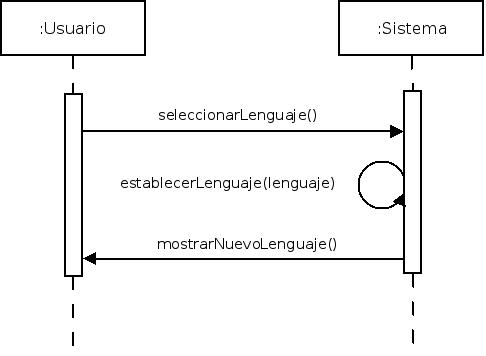
\includegraphics[scale=.55]{img/secuencias/seleccionar-idioma.jpeg}
  \caption{Diagrama de secuencia: Seleccionar lenguage}
  \label{fig:secuencia-seleccionar-lenguaje}
\end{figure}


\textbf{Contrato de operación: seleccionarLenguaje()}
\begin{itemize}
\item \textbf{Referencias cruzadas:} UC-01 (Cuadro \ref{tab:CU-idioma}).
\item \textbf{Responsabilidades:} Seleccionar un nuevo lenguaje a establecer.
\item \textbf{Precondiciones:} Ninguna
\item \textbf{Postcondiciones:}
 \begin{itemize}
\item Se selecciona un nuevo lenguaje, que el sistema utilizará para la interfaz del programa.
\end {itemize}
\end {itemize}

\textbf{Contrato de operación: establecerLenguaje(lenguaje)}
\begin{itemize}
\item \textbf{Referencias cruzadas:} UC-01 (Cuadro \ref{tab:CU-idioma}).
\item \textbf{Responsabilidades:} Establecer un nuevo lenguaje para mostrar la interfaz. Si el usuario está registrado, se establecerá como su lenguaje por defecto.
\item \textbf{Precondiciones:} 
 \begin{itemize}
\item Se ha seleccionado un lenguaje.
\end {itemize}
\item \textbf{Postcondiciones:} 
 \begin{itemize}
\item Establecer el lenguaje recibido como lenguaje para la interfaz.
\item Establecer el lenguaje por defecto para el usuario en caso de haberse identificado.
\end {itemize}
\end {itemize}


\textbf{Contrato de operación: mostrarNuevoLenguaje()}
\begin{itemize}
\item \textbf{Referencias cruzadas:} UC-01 (Cuadro \ref{tab:CU-idioma}).
\item \textbf{Responsabilidades:} Mostrar la interfaz con el nuevo lenguaje establecido.
\item \textbf{Precondiciones:} 
 \begin{itemize}
\item Se ha seleccionado y establecido un lenguaje.
\end {itemize}
\item \textbf{Postcondiciones:} 
 \begin{itemize}
\item La interfaz se muestra en el idioma seleccionado.
\end {itemize}
\end {itemize}

\vspace{10mm}

\begin{figure}[H]
\centering
  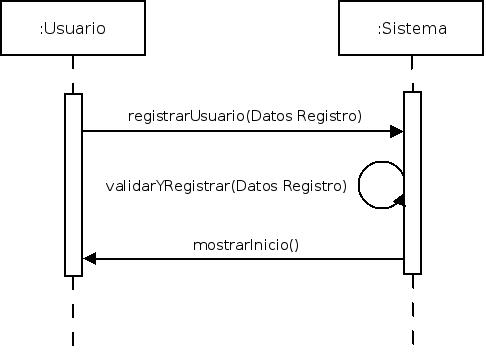
\includegraphics[scale=.55]{img/secuencias/gestion-usuarios-registro.jpeg}
  \caption{Diagrama de secuencia: Gestión de usuarios: Registro de nuevo usuario}
  \label{fig:secuencia-gestion-usuarios-registro}
\end{figure}


\textbf{Contrato de operación: registrarUsuario(Datos Registro)}
\begin{itemize}
\item \textbf{Referencias cruzadas:} UC-02 (Cuadro \ref{tab:CU-registro}).
\item \textbf{Responsabilidades:} Se mandarán los datos de registro de un nuevo usuario al sistema.
\item \textbf{Precondiciones:} Ninguna.
\item \textbf{Postcondiciones:} 
 \begin{itemize}
\item Se mandan los datos pedidos para registrar a un nuevo usuario al sistema.
\end {itemize}
\end {itemize}


\textbf{Contrato de operación: validarYRegistrar(Datos Registro)}
\begin{itemize}
\item \textbf{Referencias cruzadas:} UC-02 (Cuadro \ref{tab:CU-registro}).
\item \textbf{Responsabilidades:} Se validarán los datos recibidos y se realizará el registro del nuevo cliente.
\item \textbf{Precondiciones:} 
 \begin{itemize}
\item El usuario ha de haber enviado el formulario de registro con sus datos.
\end {itemize}
\item \textbf{Postcondiciones:} 
 \begin{itemize}
\item Se valida que los datos recibidos incluyen, al menos, todos los obligatorios.
\item Validación del email a registrar. No puede coincidir con el de algún usuario existente.
\item Registro de un nuevo usuario en el sistema.
\item Se realizará un inicio de sesión del nuevo usuario.
\end {itemize}
\end {itemize}

\textbf{Contrato de operación: mostrarInicio()}
\begin{itemize}
\item \textbf{Referencias cruzadas:} UC-02 (Cuadro \ref{tab:CU-registro}).
\item \textbf{Responsabilidades:} Se navegará hasta la página de inicio de la aplicación web.
\item \textbf{Precondiciones:} 
 \begin{itemize}
\item El usuario ha sido registrado correctamente.
\item El sistema ha iniciado sesión con los datos del usuario.
\end {itemize}
\item \textbf{Postcondiciones:} 
 \begin{itemize}
\item Se muestra la pantalla de inicio del sistema, con los datos del usuario.
\end {itemize}
\end {itemize}

\vspace{10mm}

\begin{figure}[H]
\centering
  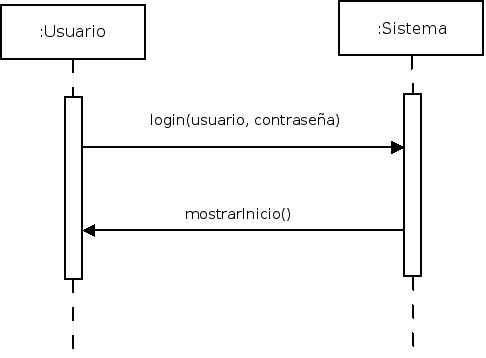
\includegraphics[scale=.55]{img/secuencias/gestion-usuarios-login.jpeg}
  \caption{Diagrama de secuencia: Iniciar sesión}
  \label{fig:secuencia-gestion-usuarios-login}
\end{figure}


\textbf{Contrato de operación: login(usuario, contraseña)}
\begin{itemize}
\item \textbf{Referencias cruzadas:} UC-03 (Cuadro \ref{tab:CU-login}).
\item \textbf{Responsabilidades:} Realizar el login del usuario en el sistema.
\item \textbf{Precondiciones:} 
 \begin{itemize}
\item El usuario no ha iniciado sesión previamente.
\end {itemize}
\item \textbf{Postcondiciones:} 
 \begin{itemize}
\item El sistema habrá comprobado que los datos de accesos son correctos.
\item Se realiza el inicio de la sesión del usuario, quedando este identificado.
\end {itemize}
\end {itemize}

\textbf{Contrato de operación: mostrarInicio()}
\begin{itemize}
\item \textbf{Referencias cruzadas:} UC-03 (Cuadro \ref{tab:CU-login}).
\item \textbf{Responsabilidades:} Se navegará hasta la página de inicio de la aplicación web.
\item \textbf{Precondiciones:} 
 \begin{itemize}
\item El usuario ha sido registrado correctamente.
\item El sistema ha iniciado sesión con los datos del usuario.
\end {itemize}
\item \textbf{Postcondiciones:} 
 \begin{itemize}
\item Se muestra la pantalla de inicio del sistema, con los datos del usuario.
\end {itemize}
\end {itemize}


\vspace{10mm}

\begin{figure}[H]
\centering
  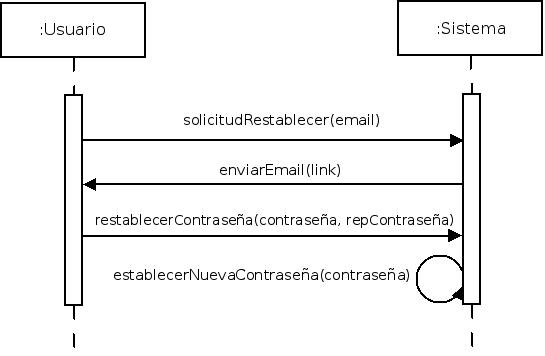
\includegraphics[scale=.55]{img/secuencias/gestion-usuarios-restablecer-contrasena.jpeg}
  \caption{Diagrama de secuencia: Restablecer contraseña}
  \label{fig:secuencia-gestion-usuarios-restablecer-contrasena}
\end{figure}


\textbf{Contrato de operación: solicitudRestablecer(email)}
\begin{itemize}
\item \textbf{Referencias cruzadas:} UC-04 (Cuadro \ref{tab:CU-restablecer-contrasena}).
\item \textbf{Responsabilidades:} Se solicitará al sistema restablecer la contraseña de un usuario que no ha iniciado sesión.
\item \textbf{Precondiciones:} 
 \begin{itemize}
\item El usuario no ha iniciado sesión previamente.
\end {itemize}
\item \textbf{Postcondiciones:} 
 \begin{itemize}
\item Se manda una solicitud de restablecer contraseña al sistema.
\end {itemize}
\end {itemize}

\textbf{Contrato de operación: enviarEmail(link)}
\begin{itemize}
\item \textbf{Referencias cruzadas:} UC-04 (Cuadro \ref{tab:CU-restablecer-contrasena}).
\item \textbf{Responsabilidades:} Se enviará un email al usuario con el enlace para establecer una nueva contraseña.
\item \textbf{Precondiciones:} 
 \begin{itemize}
\item El usuario debe estar registrado en el sistema.
\end {itemize}
\item \textbf{Postcondiciones:} 
 \begin{itemize}
\item Se comprobará que el email pertenece a un usuario registrado.
\item Se envía un email a su correo con el enlace correspondiente para establecer la nueva contraseña.
\end {itemize}
\end {itemize}

\textbf{Contrato de operación: restablecerContraseña(contraseña, repContraseña)}
\begin{itemize}
\item \textbf{Referencias cruzadas:} UC-04 (Cuadro \ref{tab:CU-restablecer-contrasena}).
\item \textbf{Responsabilidades:} Se mandará al sistema una nueva contraseña para el usuario.
\item \textbf{Precondiciones:} Ninguna.
\item \textbf{Postcondiciones:} 
 \begin{itemize}
\item El sistema comprobará que las contraseñas introducidas coinciden.
\end {itemize}
\end {itemize}

\textbf{Contrato de operación: establecerNuevaContraseña(contraseña)}
\begin{itemize}
\item \textbf{Referencias cruzadas:} UC-04 (Cuadro \ref{tab:CU-restablecer-contrasena}).
\item \textbf{Responsabilidades:} Se establecerá una nueva contraseña para el usuario.
\item \textbf{Precondiciones:} 
 \begin{itemize}
\item Se ha introducido la contraseña a establecer como nueva.
\end {itemize}
\item \textbf{Postcondiciones:} 
 \begin{itemize}
\item Se establece la contraseña introducida en la cuenta del usuario.
\item Se inicia sesión con los datos del usuario. 
\end {itemize}
\end {itemize}


\vspace{10mm}

\begin{figure}[H]
\centering
  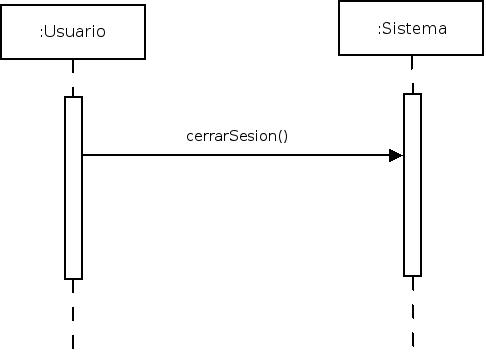
\includegraphics[scale=.55]{img/secuencias/gestion-usuarios-cerrar-sesion.jpeg}
  \caption{Diagrama de secuencia: Cerrar sesión}
  \label{fig:secuencia-gestion-usuarios-cerrar-sesion}
\end{figure}

\textbf{Contrato de operación: cerrarSesion()}
\begin{itemize}
\item \textbf{Referencias cruzadas:} UC-05 (Cuadro \ref{tab:CU-cerrar-sesion}).
\item \textbf{Responsabilidades:} Se cerrará sesión del usuario actualmente identificado.
\item \textbf{Precondiciones:} 
 \begin{itemize}
\item El usuario se ha identificado en el sistema previamente.
\end {itemize}
\item \textbf{Postcondiciones:} 
 \begin{itemize}
\item El sistema terminará la sesión del usuario.
\item La vista actual será redirigida a la página de login.
\end {itemize}
\end {itemize}


\vspace{10mm}

\begin{figure}[H]
\centering
  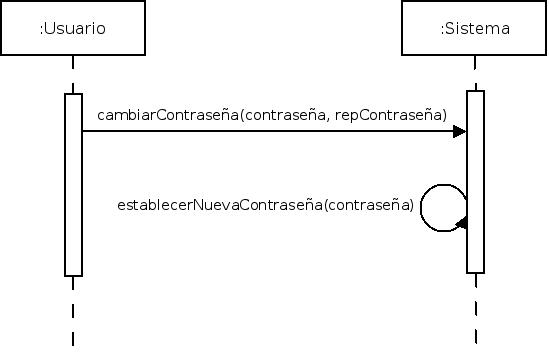
\includegraphics[scale=.55]{img/secuencias/gestion-usuarios-cambiar-contrasena.jpeg}
  \caption{Diagrama de secuencia: Cambiar contraseña}
  \label{fig:secuencia-gestion-usuarios-cambiar-contrasena}
\end{figure}

\textbf{Contrato de operación: cambiarContraseña(contraseña, repContraseña)}
\begin{itemize}
\item \textbf{Referencias cruzadas:} UC-06 (Cuadro \ref{tab:CU-cambiar-contrasena}).
\item \textbf{Responsabilidades:} Se mandará al sistema una nueva contraseña para el usuario.
\item \textbf{Precondiciones:} 
 \begin{itemize}
\item El usuario se ha identificado en el sistema previamente.
\end {itemize}
\item \textbf{Postcondiciones:} 
 \begin{itemize}
\item El sistema comprobará que las contraseñas introducidas coinciden.
\end {itemize}
\end {itemize}

\textbf{Contrato de operación: establecerNuevaContraseña(contraseña)}
\begin{itemize}
\item \textbf{Referencias cruzadas:} UC-06 (Cuadro \ref{tab:CU-cambiar-contrasena}).
\item \textbf{Responsabilidades:} Se establecerá una nueva contraseña para el usuario.
\item \textbf{Precondiciones:} 
 \begin{itemize}
\item Se ha introducido la contraseña a establecer como nueva.
\end {itemize}
\item \textbf{Postcondiciones:} 
 \begin{itemize}
\item Se establece la contraseña introducida en la cuenta del usuario.
\end {itemize}
\end {itemize}


\vspace{10mm}

\begin{figure}[H]
\centering
  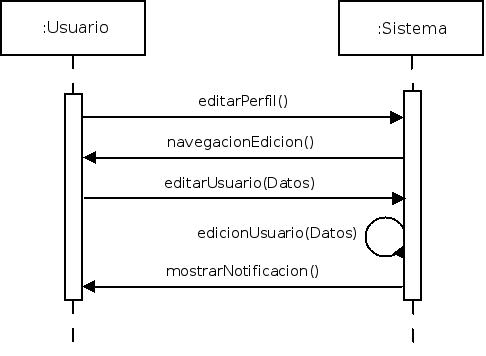
\includegraphics[scale=.55]{img/secuencias/gestion-usuarios-editar-perfil.jpeg}
  \caption{Diagrama de secuencia: Gestión de usuarios: Editar perfil}
  \label{fig:secuencia-gestion-usuarios-editar-perfil}
\end{figure}

\textbf{Contrato de operación: editarPerfil()}
\begin{itemize}
\item \textbf{Referencias cruzadas:} UC-07 (Cuadro \ref{tab:CU-editar-perfil}).
\item \textbf{Responsabilidades:} El usuario enviará al sistema la opción de editar su perfil.
\item \textbf{Precondiciones:} 
 \begin{itemize}
\item El usuario se ha identificado en el sistema previamente.
\item El usuario ha navegado hasta la pantalla de su perfil.
\end {itemize}
\item \textbf{Postcondiciones:} 
 \begin{itemize}
\item Se manda la solicitud de edición del perfil.
\end {itemize}
\end {itemize}

\textbf{Contrato de operación: navegacionEdicion()}
\begin{itemize}
\item \textbf{Referencias cruzadas:} UC-07 (Cuadro \ref{tab:CU-editar-perfil}).
\item \textbf{Responsabilidades:} El sistema mostrará la página correspondiente a la edición de los datos del perfil del usuario.
\item \textbf{Precondiciones:} 
 \begin{itemize}
\item Se ha realizado la acción correspondiente para activar la navegación.
\end {itemize}
\item \textbf{Postcondiciones:} 
 \begin{itemize}
\item Se mostrará la página de edición del perfil del usuario.
\end {itemize}
\end {itemize}

\textbf{Contrato de operación: editarUsuario(Datos)}
\begin{itemize}
\item \textbf{Referencias cruzadas:} UC-07 (Cuadro \ref{tab:CU-editar-perfil}).
\item \textbf{Responsabilidades:} Se mandará al sistema los datos del usuario para que este sea editado.
\item \textbf{Precondiciones:} 
 \begin{itemize}
\item El usuario se ha identificado en el sistema previamente.
\end {itemize}
\item \textbf{Postcondiciones:} 
 \begin{itemize}
\item Se envía el formulario de datos del perfil al sistema.
\end {itemize}
\end {itemize}

\textbf{Contrato de operación: edicionUsuario(Datos)}
\begin{itemize}
\item \textbf{Referencias cruzadas:} UC-07 (Cuadro \ref{tab:CU-editar-perfil}).
\item \textbf{Responsabilidades:} Se realizará la edición de los datos del usuario, guardándolos en el sistema.
\item \textbf{Precondiciones:} 
 \begin{itemize}
\item Se ha enviado el formulario con los datos a editar.
\end {itemize}
\item \textbf{Postcondiciones:} 
 \begin{itemize}
\item El sistema guarda los datos recibidos del usuario en la base de datos.
\end {itemize}
\end {itemize}

\textbf{Contrato de operación: mostrarNotificacion()}
\begin{itemize}
\item \textbf{Referencias cruzadas:} UC-07 (Cuadro \ref{tab:CU-editar-perfil}).
\item \textbf{Responsabilidades:} Se mostrará un mensaje de acción por pantalla.
\item \textbf{Precondiciones:} 
 \begin{itemize}
\item Se ha realizado la acción correspondiente para activar el mensaje.
\end {itemize}
\item \textbf{Postcondiciones:} 
 \begin{itemize}
\item Se muestra el mensaje correspondiente a la acción en la pantalla, a modo de notificación para el usuario. Este puede ser confirmación de la acción o algún tipo de error en la ejecución de la misma.
\end {itemize}
\end {itemize}


\vspace{10mm}

\begin{figure}[H]
\centering
  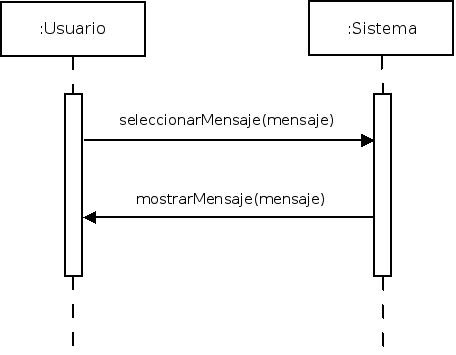
\includegraphics[scale=.55]{img/secuencias/gestion-servicios-leer-correo.jpeg}
  \caption{Diagrama de secuencia: Leer correo interno}
  \label{fig:secuencia-gestion-servicios-leer-correo}
\end{figure}

\textbf{Contrato de operación: seleccionarMensaje(mensaje)}
\begin{itemize}
\item \textbf{Referencias cruzadas:} UC-08 (Cuadro \ref{tab:CU-leer-correo}).
\item \textbf{Responsabilidades:} Se seleccionará el mensaje a mostrar.
\item \textbf{Precondiciones:} 
 \begin{itemize}
\item El usuario se ha identificado en el sistema previamente.
\end {itemize}
\item \textbf{Postcondiciones:} 
 \begin{itemize}
\item El sistema recibirá el mensaje concreto a mostrar.
\end {itemize}
\end {itemize}

\textbf{Contrato de operación: mostrarMensaje(mensaje)}
\begin{itemize}
\item \textbf{Referencias cruzadas:} UC-08 (Cuadro \ref{tab:CU-leer-correo}).
\item \textbf{Responsabilidades:} Se mostrará el mensaje seleccionado al usuario.
\item \textbf{Precondiciones:} 
 \begin{itemize}
\item El mensaje habrá sido seleccionado por el usuario previamente.
\end {itemize}
\item \textbf{Postcondiciones:} 
 \begin{itemize}
\item El sistema muestra la página de visualización de mensajes con los datos detallados del mismo.
\end {itemize}
\end {itemize}


\vspace{10mm}

\begin{figure}[H]
\centering
  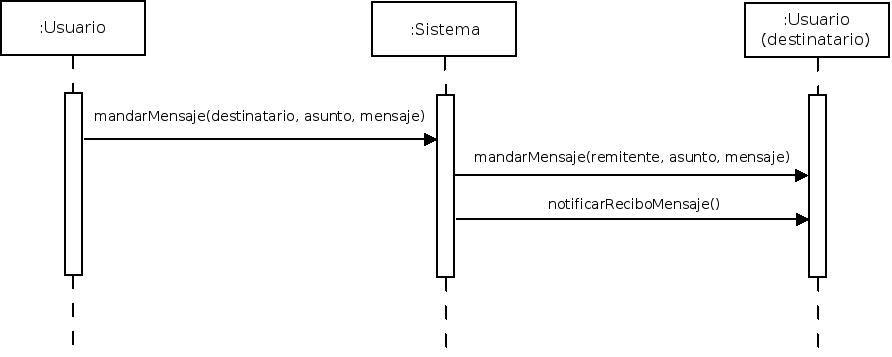
\includegraphics[scale=.45]{img/secuencias/gestion-servicios-mandar-correo.jpeg}
  \caption{Diagrama de secuencia: Mandar correo interno}
  \label{fig:secuencia-gestion-servicios-mandar-correo}
\end{figure}

\textbf{Contrato de operación: mandarMensaje(destinatario, asunto, mensaje)}
\begin{itemize}
\item \textbf{Referencias cruzadas:} UC-09 (Cuadro \ref{tab:CU-mandar-correo}).
\item \textbf{Responsabilidades:} Se mandará al sistema el mensaje que se desea enviar, junto al asunto y el destinatario.
\item \textbf{Precondiciones:} 
 \begin{itemize}
\item El usuario se ha identificado en el sistema previamente.
\end {itemize}
\item \textbf{Postcondiciones:} 
 \begin{itemize}
\item El sistema recibirá los datos del mensaje: El cuerpo (mensaje en sí), asunto y destinatario).
\end {itemize}
\end {itemize}

\textbf{Contrato de operación: mandarMensaje(remitente, asunto, mensaje)}
\begin{itemize}
\item \textbf{Referencias cruzadas:} UC-09 (Cuadro \ref{tab:CU-mandar-correo}).
\item \textbf{Responsabilidades:} El sistema mandará el mensaje recibido a su destinatario.
\item \textbf{Precondiciones:} 
 \begin{itemize}
\item Se ha recibido el mensaje por parte del remitente.
\end {itemize}
\item \textbf{Postcondiciones:} 
 \begin{itemize}
\item El sistema manda al destinatario el mensaje recibido.
\end {itemize}
\end {itemize}

\textbf{Contrato de operación: notificarReciboMensaje()}
\begin{itemize}
\item \textbf{Referencias cruzadas:} UC-09 (Cuadro \ref{tab:CU-mandar-correo}).
\item \textbf{Responsabilidades:} Notificar al destinatario del mensaje que ha recibido un correo interno.
\item \textbf{Precondiciones:} 
 \begin{itemize}
\item El usuario ha mandado un correo al usuario.
\end {itemize}
\item \textbf{Postcondiciones:} 
 \begin{itemize}
\item Se creará una nueva notificación de recibo de mensaje para el destinatario.
\end {itemize}
\end {itemize}


\vspace{10mm}

\begin{figure}[H]
\centering
  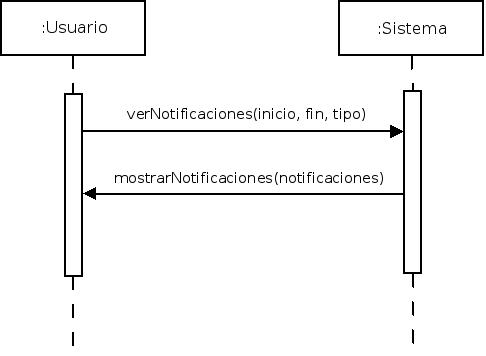
\includegraphics[scale=.50]{img/secuencias/notificaciones.jpeg}
  \caption{Diagrama de secuencia: Notificaciones}
  \label{fig:secuencia-notificaciones}
\end{figure}

\textbf{Contrato de operación: verNotificaciones(inicio, fin, tipo)}
\begin{itemize}
\item \textbf{Referencias cruzadas:} UC-10 (Cuadro \ref{tab:CU-notificaciones}).
\item \textbf{Responsabilidades:} Solicitar las notificaciones destinadas al usuario en unas determinadas fechas.
\item \textbf{Precondiciones:} 
 \begin{itemize}
\item El usuario se ha identificado en el sistema previamente.
\end {itemize}
\item \textbf{Postcondiciones:} 
 \begin{itemize}
\item Se envía al sistema el formulario con las fechas de inicio y fin elegidas para ver las notificaciones del usuario en el sistema. Se podrá mandar el tipo de notificación específica a mostrar.
\end {itemize}
\end {itemize}

\textbf{Contrato de operación: mostrarNotificaciones(notificaciones)}
\begin{itemize}
\item \textbf{Referencias cruzadas:} UC-10 (Cuadro \ref{tab:CU-notificaciones}).
\item \textbf{Responsabilidades:} Mostrar las notificaciones destinadas al usuario.
\item \textbf{Precondiciones:} 
 \begin{itemize}
\item El usuario ha solicitado ver sus notificaciones.
\end {itemize}
\item \textbf{Postcondiciones:} 
 \begin{itemize}
\item Se muestra el listado de notificaciones para el usuario entre las fechas seleccionadas.
\end {itemize}
\end {itemize}


\vspace{10mm}

\begin{figure}[H]
\centering
  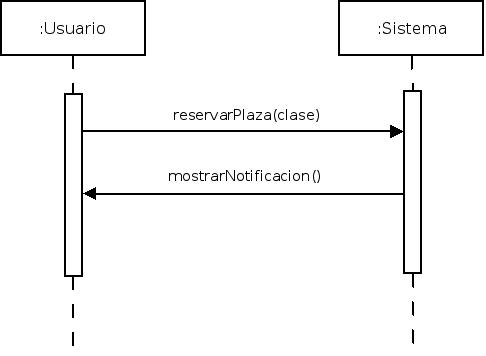
\includegraphics[scale=.55]{img/secuencias/gestion-servicios-reservar-clase.jpeg}
  \caption{Diagrama de secuencia: Gestión de servicios: Reservar plaza en una clase}
  \label{fig:secuencia-gestion-servicios-reservar-clase}
\end{figure}

\textbf{Contrato de operación: reservarPlaza(clase)}
\begin{itemize}
\item \textbf{Referencias cruzadas:} UC-11 (Cuadro \ref{tab:CU-reservar-clase}).
\item \textbf{Responsabilidades:} Se reservará una plaza de la clase seleccionada al usuario.
\item \textbf{Precondiciones:} 
 \begin{itemize}
\item El usuario se ha identificado en el sistema previamente.
\item Ha de haber al menos una plaza libre en la clase.
\item El usuario no posee plaza en la clase seleccionada.
\end {itemize}
\item \textbf{Postcondiciones:} 
 \begin{itemize}
\item Se reservará una plaza de la clase seleccionada al usuario.
\item Se reduce la plaza reservada de las totales disponibles de la clase.
\end {itemize}
\end {itemize}

\textbf{Contrato de operación: mostrarNotificacion()}
\begin{itemize}
\item \textbf{Referencias cruzadas:} UC-11 (Cuadro \ref{tab:CU-reservar-clase}).
\item \textbf{Responsabilidades:} Se mostrará un mensaje de acción por pantalla.
\item \textbf{Precondiciones:} 
 \begin{itemize}
\item Se ha realizado la acción correspondiente para activar el mensaje.
\end {itemize}
\item \textbf{Postcondiciones:} 
 \begin{itemize}
\item Se muestra el mensaje correspondiente a la acción en la pantalla, a modo de notificación para el usuario. Este puede ser confirmación de la acción o algún tipo de error en la ejecución de la misma.
\end {itemize}
\end {itemize}


\vspace{10mm}

\begin{figure}[H]
\centering
  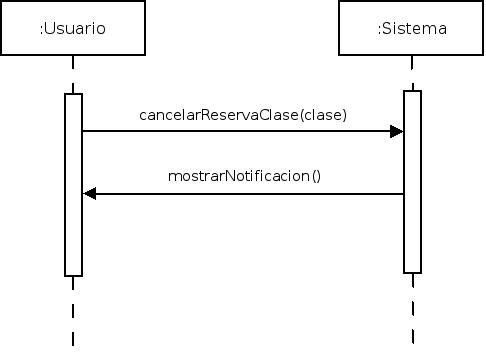
\includegraphics[scale=.55]{img/secuencias/gestion-servicios-cancelar-reserva-clase.jpeg}
  \caption{Diagrama de secuencia: Gestión de servicios: Cancelación de reserva de una clase}
  \label{fig:secuencia-gestion-servicios-cancelar-reserva-clase}
\end{figure}

\textbf{Contrato de operación: cancelarReservaClase(clase)}
\begin{itemize}
\item \textbf{Referencias cruzadas:} UC-12 (Cuadro \ref{tab:CU-cancelar-reserva-clase}).
\item \textbf{Responsabilidades:} Se cancelará la reserva del usuario previamente realizada de una clase específica.
\item \textbf{Precondiciones:} 
 \begin{itemize}
\item El usuario se ha identificado en el sistema previamente.
\item La clase ha sido reservada previamente.
\end {itemize}
\item \textbf{Postcondiciones:} 
 \begin{itemize}
\item Se cancela la reserva de la plaza del usuario en la clase específica.
\item Las plazas disponibles de la clase en concreto se incrementan en uno.
\end {itemize}
\end {itemize}

\textbf{Contrato de operación: mostrarNotificacion()}
\begin{itemize}
\item \textbf{Referencias cruzadas:} UC-12 (Cuadro \ref{tab:CU-cancelar-reserva-clase}).
\item \textbf{Responsabilidades:} Se mostrará un mensaje de acción por pantalla.
\item \textbf{Precondiciones:} 
 \begin{itemize}
\item Se ha realizado la acción correspondiente para activar el mensaje.
\end {itemize}
\item \textbf{Postcondiciones:} 
 \begin{itemize}
\item Se muestra el mensaje correspondiente a la acción en la pantalla, a modo de notificación para el usuario. Este puede ser confirmación de la acción o algún tipo de error en la ejecución de la misma.
\end {itemize}
\end {itemize}


\vspace{10mm}

\begin{figure}[H]
\centering
  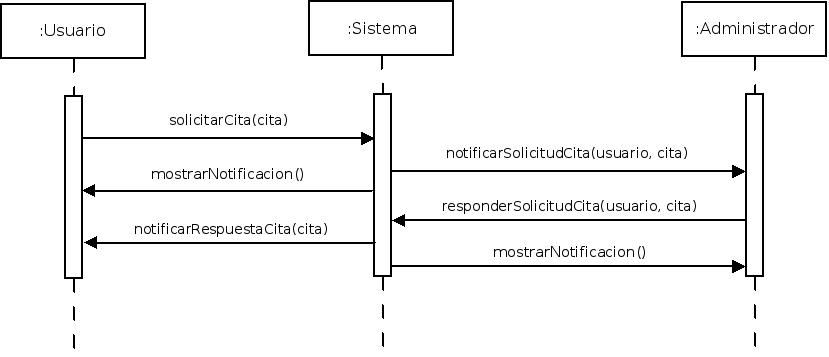
\includegraphics[scale=.45]{img/secuencias/gestion-servicios-solicitar-responder-cita.jpeg}
  \caption{Diagrama de secuencia:: Gestión de servicios: Solicitud de cita y respuesta}
  \label{fig:secuencia-gestion-servicios-solicitar-responder-cita.jpeg}
\end{figure}

\textbf{Contrato de operación: solicitarCita(cita)}
\begin{itemize}
\item \textbf{Referencias cruzadas:} UC-13 (Cuadro \ref{tab:CU-solicitar-cita}), UC-14 (Cuadro \ref{tab:CU-responder-solicitud-cita}).
\item \textbf{Responsabilidades:} Se enviará una solicitud de la cita seleccionada a los administradores.
\item \textbf{Precondiciones:} 
 \begin{itemize}
\item El usuario se ha identificado en el sistema previamente.
\item La cita debe estar disponible para su solicitud.
\end {itemize}
\item \textbf{Postcondiciones:} 
 \begin{itemize}
\item Se enviará una solicitud de la cita seleccionada a los administradores.
\item Se establece la cita como no disponible hasta que se resuelva la solicitud.
\end {itemize}
\end {itemize}

\textbf{Contrato de operación: notificarSolicitudCita(usuario, cita)}
\begin{itemize}
\item \textbf{Referencias cruzadas:} UC-13 (Cuadro \ref{tab:CU-solicitar-cita}), UC-14 (Cuadro \ref{tab:CU-responder-solicitud-cita}).
\item \textbf{Responsabilidades:} Mandar una notificación de solicitud de cita de un determinado usuario a los administradores.
\item \textbf{Precondiciones:} 
 \begin{itemize}
\item Se ha recibido una solicitud de cita en el sistema.
\end {itemize}
\item \textbf{Postcondiciones:} 
 \begin{itemize}
\item Se creará una nueva notificación de solicitud de cita para los administradores.
\end {itemize}
\end {itemize}

\textbf{Contrato de operación: mostrarNotificacion()}
\begin{itemize}
\item \textbf{Referencias cruzadas:} UC-13 (Cuadro \ref{tab:CU-solicitar-cita}), UC-14 (Cuadro \ref{tab:CU-responder-solicitud-cita}).
\item \textbf{Responsabilidades:} Se mostrará un mensaje de acción por pantalla.
\item \textbf{Precondiciones:} 
 \begin{itemize}
\item Se ha realizado la acción correspondiente para activar el mensaje.
\end {itemize}
\item \textbf{Postcondiciones:} 
 \begin{itemize}
\item Se muestra el mensaje correspondiente a la acción en la pantalla, a modo de notificación para el usuario. Este puede ser confirmación de la acción o algún tipo de error en la ejecución de la misma.
\end {itemize}
\end {itemize}

\textbf{Contrato de operación: responderSolicitudCita(usuario, cita)}
\begin{itemize}
\item \textbf{Referencias cruzadas:} UC-13 (Cuadro \ref{tab:CU-solicitar-cita}), UC-14 (Cuadro \ref{tab:CU-responder-solicitud-cita}).
\item \textbf{Responsabilidades:} Responder a la solicitud de cita recibida por parte de un usuario específico.
\item \textbf{Precondiciones:} 
 \begin{itemize}
\item El administrador se ha identificado en el sistema previamente.
\item Se ha recibido una solicitud de cita por parte de un determinado usuario.
\end {itemize}
\item \textbf{Postcondiciones:} 
 \begin{itemize}
\item Se envía la respuesta de la solicitud al sistema.
\item Dependiendo de la respuesta (declinada o aceptada), se establece la disponibilidad de la cita (disponible o no disponible).
\end {itemize}
\end {itemize}

\textbf{Contrato de operación: notificarRespuestaCita(cita)}
\begin{itemize}
\item \textbf{Referencias cruzadas:} UC-13 (Cuadro \ref{tab:CU-solicitar-cita}), UC-14 (Cuadro \ref{tab:CU-responder-solicitud-cita}).
\item \textbf{Responsabilidades:} Mandar una notificación de respuesta de la solicitud de cita al usuario.
\item \textbf{Precondiciones:} 
 \begin{itemize}
\item Se ha recibido una respuesta de la solicitud de cita por parte de los administradores.
\end {itemize}
\item \textbf{Postcondiciones:} 
 \begin{itemize}
\item Se creará una nueva notificación de repuesta de solicitud de cita para el usuario.
\end {itemize}
\end {itemize}


\vspace{10mm}

\begin{figure}[H]
\centering
  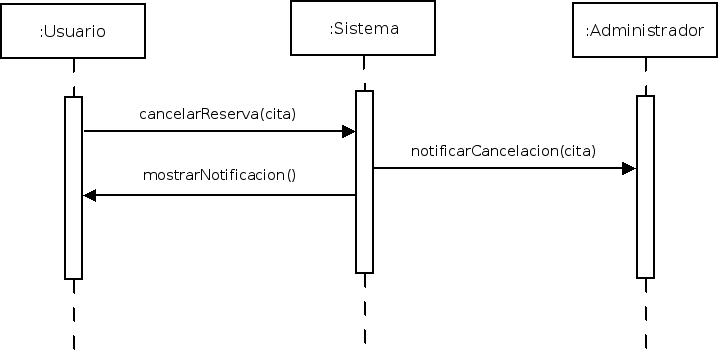
\includegraphics[scale=.50]{img/secuencias/gestion-servicios-cancelar-cita-por-parte-de-usuario.jpeg}
  \caption{Diagrama de secuencia: Gestión de servicios: Cancelar Cita}
  \label{fig:secuencia-gestion-servicios-cancelar-cita-por-parte-de-usuario}
\end{figure}

\textbf{Contrato de operación: cancelarReserva(cita)}
\begin{itemize}
\item \textbf{Referencias cruzadas:} UC-15 (Cuadro \ref{tab:CU-cancelar-cita}).
\item \textbf{Responsabilidades:} Se cancelará la cita o solicitud de cita del usuario, notificando a los administradores.
\item \textbf{Precondiciones:} 
 \begin{itemize}
\item El usuario se ha identificado en el sistema previamente.
\item El usuario ha solicitado la cita.
\end {itemize}
\item \textbf{Postcondiciones:} 
 \begin{itemize}
\item Se cancela la reserva o solicitud de la cita seleccionada.
\end {itemize}
\end {itemize}

\textbf{Contrato de operación: notificarCancelacion(cita)}
\begin{itemize}
\item \textbf{Referencias cruzadas:} UC-15 (Cuadro \ref{tab:CU-cancelar-cita}).
\item \textbf{Responsabilidades:} Mandar una notificación de cancelación de la reserva o solicitud de cita a los administradores.
\item \textbf{Precondiciones:} 
 \begin{itemize}
\item Se ha cancelado una solicitud o reserva de cita.
\end {itemize}
\item \textbf{Postcondiciones:} 
 \begin{itemize}
\item Se creará una nueva notificación de cancelación de reserva o solicitud de cita para los administradores.
\end {itemize}
\end {itemize}

\textbf{Contrato de operación: mostrarNotificacion()}
\begin{itemize}
\item \textbf{Referencias cruzadas:} UC-15 (Cuadro \ref{tab:CU-cancelar-cita}).
\item \textbf{Responsabilidades:} Se mostrará un mensaje de acción por pantalla.
\item \textbf{Precondiciones:} 
 \begin{itemize}
\item Se ha realizado la acción correspondiente para activar el mensaje.
\end {itemize}
\item \textbf{Postcondiciones:} 
 \begin{itemize}
\item Se muestra el mensaje correspondiente a la acción en la pantalla, a modo de notificación para el usuario. Este puede ser confirmación de la acción o algún tipo de error en la ejecución de la misma.
\end {itemize}
\end {itemize}


\vspace{10mm}

\begin{figure}[H]
\centering
  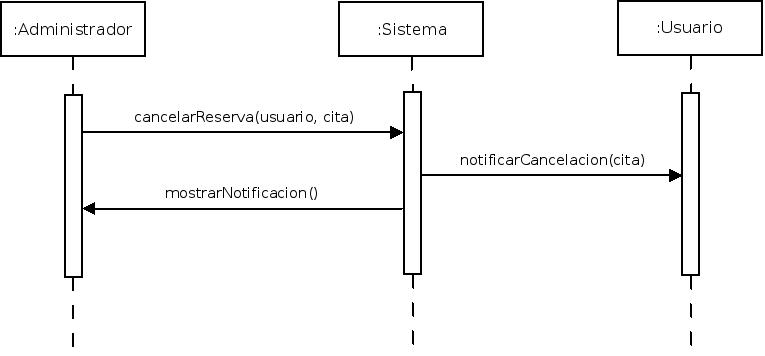
\includegraphics[scale=.50]{img/secuencias/gestion-servicios-cancelar-cita-por-parte-de-admin.jpeg}
  \caption{Diagrama de secuencia: Gestión de servicios: Cancelar cita (Administrador)}
  \label{fig:secuencia-gestion-servicios-cancelar-cita-por-parte-de-admin}
\end{figure}

\textbf{Contrato de operación: cancelarReserva(cita)}
\begin{itemize}
\item \textbf{Referencias cruzadas:} UC-16 (Cuadro \ref{tab:CU-cancelar-cita-admin}).
\item \textbf{Responsabilidades:} Un administrador cancelará la cita o solicitud de cita del usuario, notificando al mismo.
\item \textbf{Precondiciones:} 
 \begin{itemize}
\item El administrador se ha identificado en el sistema previamente.
\item El usuario ha solicitado la cita.
\end {itemize}
\item \textbf{Postcondiciones:} 
 \begin{itemize}
\item Se cancela la reserva o solicitud de la cita seleccionada.
\end {itemize}
\end {itemize}

\textbf{Contrato de operación: notificarCancelacion(cita)}
\begin{itemize}
\item \textbf{Referencias cruzadas:} UC-16 (Cuadro \ref{tab:CU-cancelar-cita-admin}).
\item \textbf{Responsabilidades:} Mandar una notificación de cancelación de la reserva o solicitud de cita al usuario.
\item \textbf{Precondiciones:} 
 \begin{itemize}
\item Se ha cancelado una solicitud o reserva de cita.
\end {itemize}
\item \textbf{Postcondiciones:} 
 \begin{itemize}
\item Se creará una nueva notificación de cancelación de reserva o solicitud de cita para el usuario.
\end {itemize}
\end {itemize}

\textbf{Contrato de operación: mostrarNotificacion()}
\begin{itemize}
\item \textbf{Referencias cruzadas:} UC-16 (Cuadro \ref{tab:CU-cancelar-cita-admin}).
\item \textbf{Responsabilidades:} Se mostrará un mensaje de acción por pantalla.
\item \textbf{Precondiciones:} 
 \begin{itemize}
\item Se ha realizado la acción correspondiente para activar el mensaje.
\end {itemize}
\item \textbf{Postcondiciones:} 
 \begin{itemize}
\item Se muestra el mensaje correspondiente a la acción en la pantalla, a modo de notificación para el administrador. Este puede ser confirmación de la acción o algún tipo de error en la ejecución de la misma.
\end {itemize}
\end {itemize}


\vspace{10mm}

\begin{figure}[H]
\centering
  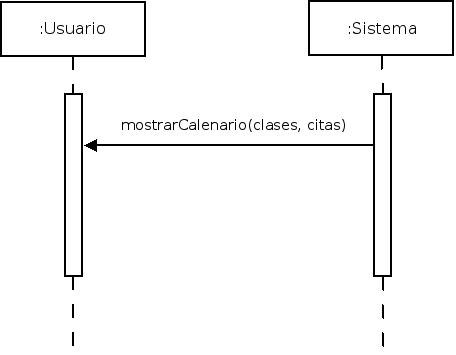
\includegraphics[scale=.55]{img/secuencias/gestion-servicios-calendario.jpeg}
  \caption{Diagrama de secuencia: Gestión de servicios: Calendario de actividades}
  \label{fig:secuencia-gestion-servicios-calendario}
\end{figure}

\textbf{Contrato de operación: mostrarCalendario(clases, citas)}
\begin{itemize}
\item \textbf{Referencias cruzadas:} UC-17 (Cuadro \ref{tab:CU-calendario}).
\item \textbf{Responsabilidades:} Mostrar el calendario mensual con las clases y citas disponibles en el sistema. Se distinguirá el estado de las mismas por su color de fondo o borde, para diferenciar entre clases o citas pasadas, disponibles, reservadas por el usuario...
\item \textbf{Precondiciones:} 
 \begin{itemize}
\item El usuario se ha identificado en el sistema previamente.
\item El usuario ha accedido a la página de visualización del calendario.
\end {itemize}
\item \textbf{Postcondiciones:} 
 \begin{itemize}
\item El sistema muestra el calendario con todas las citas y clases disponibles, distinguiendo su estado por colores. 
\end {itemize}
\end {itemize}


\vspace{10mm}

\begin{figure}[H]
\centering
  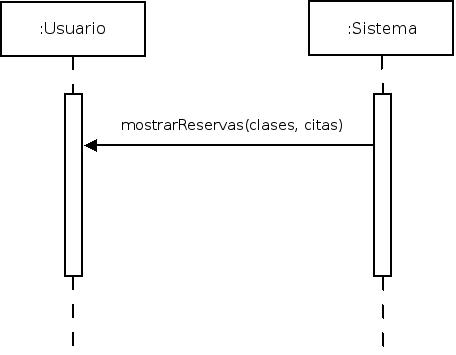
\includegraphics[scale=.55]{img/secuencias/gestion-servicios-reservas.jpeg}
  \caption{Diagrama de secuencia: Gestión de servicios: Consultar reservas}
  \label{fig:secuencia-gestion-servicios-reservas}
\end{figure}

\textbf{Contrato de operación: mostrarReservas(citas, clases)}
\begin{itemize}
\item \textbf{Referencias cruzadas:} UC-18 (Cuadro \ref{tab:CU-reservas}).
\item \textbf{Responsabilidades:} Se mostrará una lista de las citas y reservas del usuario, tanto pasadas como actuales.
\item \textbf{Precondiciones:} 
 \begin{itemize}
\item El usuario se ha identificado en el sistema previamente.
\item El usuario ha navegado hasta la página de vista de reservas.
\end {itemize}
\item \textbf{Postcondiciones:} 
 \begin{itemize}
\item Se listarán todas las citas y clases que el usuario haya reservado, distinguiendo entre pasadas y actuales.
\end {itemize}
\end {itemize}


\vspace{10mm}

\begin{figure}[H]
\centering
  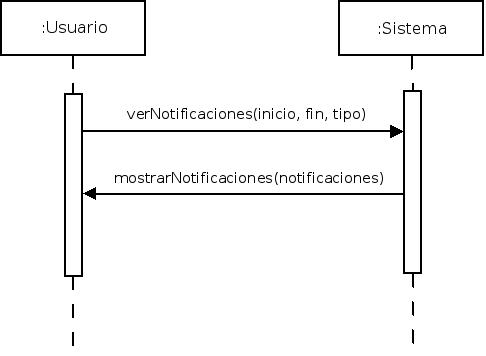
\includegraphics[scale=.55]{img/secuencias/notificaciones.jpeg}
  \caption{Diagrama de secuencia: Notificaciones}
  \label{fig:secuencia-notificaciones}
\end{figure}

\textbf{Contrato de operación: verAuditorias(inicio, fin, tipo)}
\begin{itemize}
\item \textbf{Referencias cruzadas:} UC-19 (Cuadro \ref{tab:CU-notificaciones}).
\item \textbf{Responsabilidades:} Solicitar las notificaciones que el sistema ha creado destinadas al usuario en unas determinadas fechas.
\item \textbf{Precondiciones:} 
 \begin{itemize}
\item El usuario se ha identificado en el sistema previamente.
\end {itemize}
\item \textbf{Postcondiciones:} 
 \begin{itemize}
\item Se envía al sistema el formulario con las fechas de inicio y fin elegidas para ver las notificaciones del usuario. Se podrá mandar el tipo de notificación específica a mostrar.
\end {itemize}
\end {itemize}

\textbf{Contrato de operación: mostrarNotificaciones(notificaciones)}
\begin{itemize}
\item \textbf{Referencias cruzadas:} UC-19 (Cuadro \ref{tab:CU-notificaciones}).
\item \textbf{Responsabilidades:} Se mostrará la lista de notificaciones destinadas al usuario.
\item \textbf{Precondiciones:} 
 \begin{itemize}
\item El usuario se ha identificado en el sistema previamente.
\item El usuario ha navegado hasta la vista de notificaciones.
\end {itemize}
\item \textbf{Postcondiciones:} 
 \begin{itemize}
\item Se listarán todas las notificaciones que el sistema ha creado para el usuario.
\end {itemize}
\end {itemize}


\vspace{10mm}

\begin{figure}[H]
\centering
  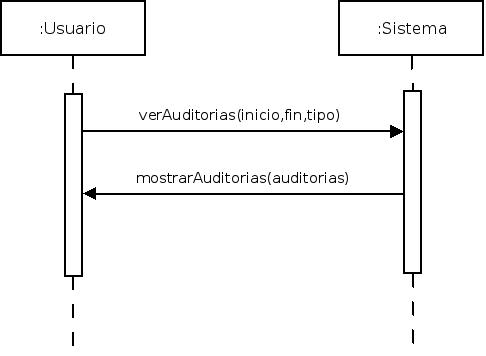
\includegraphics[scale=.55]{img/secuencias/auditorias.jpeg}
  \caption{Diagrama de secuencia: Auditorías}
  \label{fig:secuencia-auditorias}
\end{figure}

\textbf{Contrato de operación: verAuditorias(inicio, fin, tipo)}
\begin{itemize}
\item \textbf{Referencias cruzadas:} UC-20 (Cuadro \ref{tab:CU-auditorias}).
\item \textbf{Responsabilidades:} Solicitar las acciones llevadas a cabo por el usuario en unas determinadas fechas.
\item \textbf{Precondiciones:} 
 \begin{itemize}
\item El usuario se ha identificado en el sistema previamente.
\end {itemize}
\item \textbf{Postcondiciones:} 
 \begin{itemize}
\item Se envía al sistema el formulario con las fechas de inicio y fin elegidas para ver las acciones del usuario en el sistema. Se podrá mandar el tipo de acción específica a mostrar.
\end {itemize}
\end {itemize}

\textbf{Contrato de operación: mostrarAuditorias(auditorias)}
\begin{itemize}
\item \textbf{Referencias cruzadas:} UC-20 (Cuadro \ref{tab:CU-auditorias}).
\item \textbf{Responsabilidades:} Mostrar las acciones llevadas a cabo por el usuario en el sistema.
\item \textbf{Precondiciones:} 
 \begin{itemize}
\item El usuario ha solicitado ver sus auditorías.
\end {itemize}
\item \textbf{Postcondiciones:} 
 \begin{itemize}
\item Se muestra el listado de acciones realizadas entre las fechas seleccionadas.
\end {itemize}
\end {itemize}


\vspace{10mm}

\begin{figure}[H]
\centering
  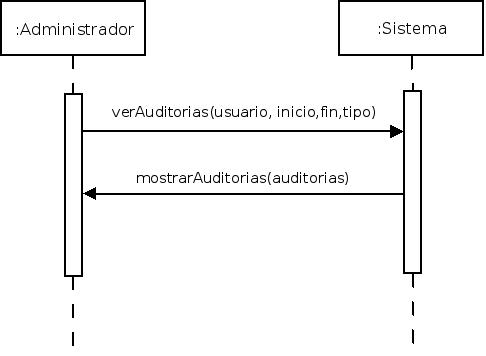
\includegraphics[scale=.55]{img/secuencias/auditorias-administrador.jpeg}
  \caption{Diagrama de secuencia: Auditorías de Administradores}
  \label{fig:secuencia-auditorias-administrador}
\end{figure}

\textbf{Contrato de operación: verAuditorias(usuario, inicio, fin, tipo)}
\begin{itemize}
\item \textbf{Referencias cruzadas:} UC-21 (Cuadro \ref{tab:CU-auditorias-admin}).
\item \textbf{Responsabilidades:} Solicitar las acciones llevadas a cabo por el usuario seleccionado en unas determinadas fechas.
\item \textbf{Precondiciones:} 
 \begin{itemize}
\item El administrador se ha identificado en el sistema previamente.
\end {itemize}
\item \textbf{Postcondiciones:} 
 \begin{itemize}
\item Se envía al sistema el formulario con el usuario específico y las fechas de inicio y fin elegidas para ver las acciones del usuario en el sistema. Se podrá mandar el tipo de acción específica a mostrar.
\end {itemize}
\end {itemize}

\textbf{Contrato de operación: mostrarAuditorias(auditorias)}
\begin{itemize}
\item \textbf{Referencias cruzadas:} UC-21 (Cuadro \ref{tab:CU-auditorias-admin}).
\item \textbf{Responsabilidades:} Mostrar las acciones llevadas a cabo por el usuario seleccionado en el sistema.
\item \textbf{Precondiciones:} 
 \begin{itemize}
\item El administrador ha solicitado ver las auditorías seleccionadas.
\end {itemize}
\item \textbf{Postcondiciones:} 
 \begin{itemize}
\item Se muestra el listado de acciones realizadas entre las fechas seleccionadas para el usuario especificado.
\end {itemize}
\end {itemize}

\vspace{10mm}

\begin{figure}[H]
\centering
  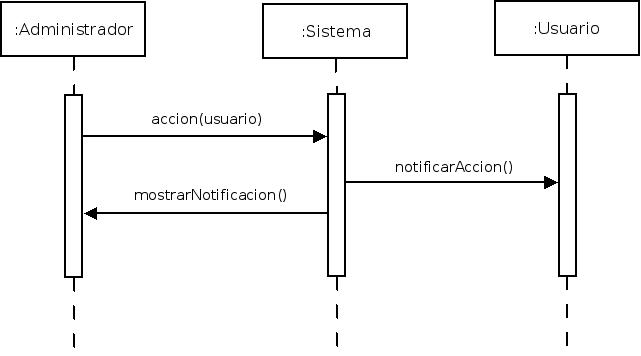
\includegraphics[scale=.50]{img/secuencias/gestion-usuarios-activar-suspender.jpeg}
  \caption{Diagrama de secuencia: Gestión de usuarios: Activar/Suspender}
  \label{fig:secuencia-gestion-usuarios-activar-suspender}
\end{figure}

\textbf{Contrato de operación: accion(usuario)}
\begin{itemize}
\item \textbf{Referencias cruzadas:} UC-22 (Cuadro \ref{tab:CU-activar-suspender-usuario}).
\item \textbf{Responsabilidades:} El administrador podrá activar o suspender al usuario seleccionado.
\item \textbf{Precondiciones:} 
 \begin{itemize}
\item El administrador se ha identificado en el sistema previamente.
\item El usuario seleccionado debe estar activo para ser suspendido o viceversa.
\end {itemize}
\item \textbf{Postcondiciones:} 
 \begin{itemize}
\item Se realizará la acción seleccionada por el administrador \textit{(activar, suspender)} referente a un usuario específico.
\end {itemize}
\end {itemize}

\textbf{Contrato de operación: notificarAccion()}
\begin{itemize}
\item \textbf{Referencias cruzadas:} UC-22 (Cuadro \ref{tab:CU-activar-suspender-usuario}).
\item \textbf{Responsabilidades:} Mandar una notificación de suspensión/activación de la cuenta al usuario.
\item \textbf{Precondiciones:} 
 \begin{itemize}
\item Se ha suspendido/activado la cuenta de un usuario.
\end {itemize}
\item \textbf{Postcondiciones:} 
 \begin{itemize}
\item Se creará una nueva notificación de activación o suspensión de cuenta para el usuario seleccionado.
\end {itemize}
\end {itemize}

\textbf{Contrato de operación: mostrarNotificacion()}
\begin{itemize}
\item \textbf{Referencias cruzadas:} UC-22 (Cuadro \ref{tab:CU-activar-suspender-usuario}).
\item \textbf{Responsabilidades:} Se mostrará un mensaje de acción por pantalla.
\item \textbf{Precondiciones:} 
 \begin{itemize}
\item Se ha realizado la acción correspondiente para activar el mensaje.
\end {itemize}
\item \textbf{Postcondiciones:} 
 \begin{itemize}
\item Se muestra el mensaje correspondiente a la acción en la pantalla, a modo de notificación para el administrador. Este puede ser confirmación de la acción o algún tipo de error en la ejecución de la misma.
\end {itemize}
\end {itemize}


\vspace{10mm}

\begin{figure}[H]
\centering
  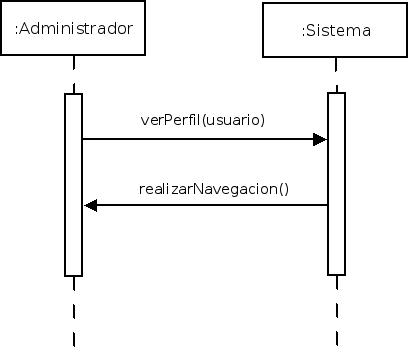
\includegraphics[scale=.55]{img/secuencias/gestion-usuarios-ver-perfil.jpeg}
  \caption{Diagrama de secuencia: Gestión de usuarios: Ver perfil (Administrador)}
  \label{fig:secuencia-gestion-usuarios-ver-perfil}
\end{figure}

\textbf{Contrato de operación: verPerfil(usuario)}
\begin{itemize}
\item \textbf{Referencias cruzadas:} UC-23 (Cuadro \ref{tab:CU-ver-perfil-admin}).
\item \textbf{Responsabilidades:} El administrador podrá ver el perfil del usuario seleccionado.
\item \textbf{Precondiciones:} 
 \begin{itemize}
\item El administrador se ha identificado en el sistema previamente.
\end {itemize}
\item \textbf{Postcondiciones:} 
 \begin{itemize}
\item Se navegará a la página correspondiente para ver los detalles del perfil de un usuario específico.
\end {itemize}
\end {itemize}

\textbf{Contrato de operación: realizarNavegacion()}
\begin{itemize}
\item \textbf{Referencias cruzadas:} UC-23 (Cuadro \ref{tab:CU-ver-perfil-admin}).
\item \textbf{Responsabilidades:} El sistema mostrará la página correspondiente al perfil del usuario.
\item \textbf{Precondiciones:} 
 \begin{itemize}
\item Se ha realizado la acción correspondiente para activar la navegación.
\end {itemize}
\item \textbf{Postcondiciones:} 
 \begin{itemize}
\item Se mostrará la página del perfil de usuario al administrador.
\end {itemize}
\end {itemize}


\vspace{10mm}

\begin{figure}[H]
\centering
  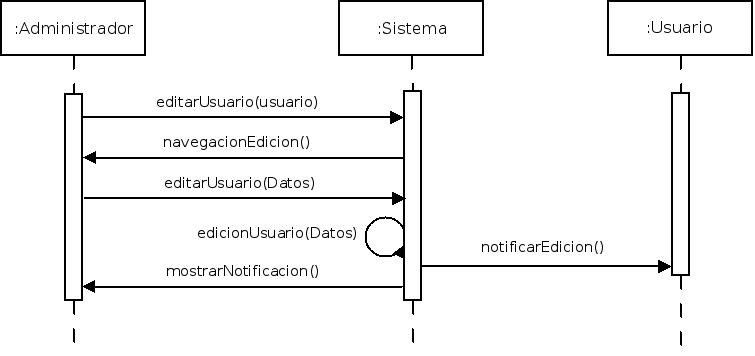
\includegraphics[scale=.50]{img/secuencias/gestion-usuarios-editar-usuario-administrador.jpeg}
  \caption{Diagrama de secuencia: Gestión de usuarios: Editar usuario (Administrador)}
  \label{fig:secuencia-gestion-usuarios-editar-usuario-administrador}
\end{figure}

\textbf{Contrato de operación: editarUsuario(usuario)}
\begin{itemize}
\item \textbf{Referencias cruzadas:} UC-24 (Cuadro \ref{tab:CU-editar-usuario-admin}).
\item \textbf{Responsabilidades:} Se informará al sistema de la acción de edición de un usuario específico.
\item \textbf{Precondiciones:} 
 \begin{itemize}
\item El administrador se ha identificado en el sistema previamente.
\end {itemize}
\item \textbf{Postcondiciones:} 
 \begin{itemize}
\item Se manda la solicitud de edición del usuario seleccionado.
\end {itemize}
\end {itemize}

\textbf{Contrato de operación: navegacionEdicion()}
\begin{itemize}
\item \textbf{Referencias cruzadas:} UC-24 (Cuadro \ref{tab:CU-editar-usuario-admin}).
\item \textbf{Responsabilidades:} El sistema mostrará la página correspondiente a la edición de los datos del usuario.
\item \textbf{Precondiciones:} 
 \begin{itemize}
\item Se ha realizado la acción correspondiente para activar la navegación.
\end {itemize}
\item \textbf{Postcondiciones:} 
 \begin{itemize}
\item Se mostrará la página de edición del perfil del usuario seleccionado.
\end {itemize}
\end {itemize}

\textbf{Contrato de operación: editarUsuario(Datos)}
\begin{itemize}
\item \textbf{Referencias cruzadas:} UC-24 (Cuadro \ref{tab:CU-editar-usuario-admin}).
\item \textbf{Responsabilidades:} Se mandará al sistema los datos del usuario para que este sea editado.
\item \textbf{Precondiciones:} 
 \begin{itemize}
\item El administrador se ha identificado en el sistema previamente.
\end {itemize}
\item \textbf{Postcondiciones:} 
 \begin{itemize}
\item Se envía el formulario de datos del cliente a editar al sistema.
\end {itemize}
\end {itemize}

\textbf{Contrato de operación: edicionUsuario(Datos)}
\begin{itemize}
\item \textbf{Referencias cruzadas:} UC-24 (Cuadro \ref{tab:CU-editar-usuario-admin}).
\item \textbf{Responsabilidades:} Se realizará la edición de los datos del usuario, guardándolos en el sistema.
\item \textbf{Precondiciones:} 
 \begin{itemize}
\item Se ha enviado el formulario con los datos a editar.
\end {itemize}
\item \textbf{Postcondiciones:} 
 \begin{itemize}
\item El sistema guarda los datos recibidos para el usuario específico en la base de datos.
\end {itemize}
\end {itemize}

\textbf{Contrato de operación: notificarEdicion()}
\begin{itemize}
\item \textbf{Referencias cruzadas:} UC-24 (Cuadro \ref{tab:CU-editar-usuario-admin}).
\item \textbf{Responsabilidades:} Mandar una notificación de edición del perfil por parte del administrador al usuario.
\item \textbf{Precondiciones:} 
 \begin{itemize}
\item Se ha editado los datos del usuario por parte del administrador.
\end {itemize}
\item \textbf{Postcondiciones:} 
 \begin{itemize}
\item Se creará una nueva notificación de edición del perfil para el usuario seleccionado, indicando quién lo ha modificado.
\end {itemize}
\end {itemize}

\textbf{Contrato de operación: mostrarNotificacion()}
\begin{itemize}
\item \textbf{Referencias cruzadas:} UC-24 (Cuadro \ref{tab:CU-editar-usuario-admin}).
\item \textbf{Responsabilidades:} Se mostrará un mensaje de acción por pantalla.
\item \textbf{Precondiciones:} 
 \begin{itemize}
\item Se ha realizado la acción correspondiente para activar el mensaje.
\end {itemize}
\item \textbf{Postcondiciones:} 
 \begin{itemize}
\item Se muestra el mensaje correspondiente a la acción en la pantalla, a modo de notificación para el administrador. Este puede ser confirmación de la acción o algún tipo de error en la ejecución de la misma.
\end {itemize}
\end {itemize}


\vspace{10mm}

\begin{figure}[H]
\centering
  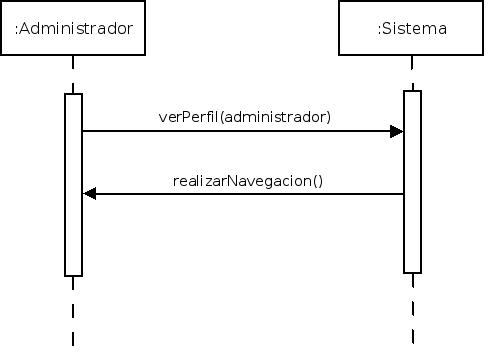
\includegraphics[scale=.55]{img/secuencias/gestion-administradores-ver-perfil.jpeg}
  \caption{Diagrama de secuencia: Gestión de administradores: Ver perfil de administrador}
  \label{fig:secuencia-gestion-administradores-ver-perfil}
\end{figure}

\textbf{Contrato de operación: verPerfil(administrador)}
\begin{itemize}
\item \textbf{Referencias cruzadas:} UC-25 (Cuadro \ref{tab:CU-ver-perfil-de-admin}).
\item \textbf{Responsabilidades:} El administrador podrá ver el perfil de otro administrador seleccionado.
\item \textbf{Precondiciones:} 
 \begin{itemize}
\item El administrador se ha identificado en el sistema previamente.
\end {itemize}
\item \textbf{Postcondiciones:} 
 \begin{itemize}
\item Se navegará a la página del perfil del administrador seleccionado para ver sus detalles en el sistema.
\end {itemize}
\end {itemize}

\textbf{Contrato de operación: realizarNavegacion()}
\begin{itemize}
\item \textbf{Referencias cruzadas:} UC-25 (Cuadro \ref{tab:CU-ver-perfil-de-admin}).
\item \textbf{Responsabilidades:} El sistema mostrará la página correspondiente a la opción seleccionada para realizar la acción (ver administrador o mandar un mensaje al administrador).
\item \textbf{Precondiciones:} 
 \begin{itemize}
\item Se ha realizado la acción correspondiente para activar la navegación.
\end {itemize}
\item \textbf{Postcondiciones:} 
 \begin{itemize}
\item Se mostrará la página correspondiente a la opción seleccionada por el administrador para realizar la acción \textit{(ver perfil de administrador o mandar un correo al administrador)}.
\end {itemize}
\end {itemize}

\vspace{10mm}

\begin{figure}[H]
\centering
  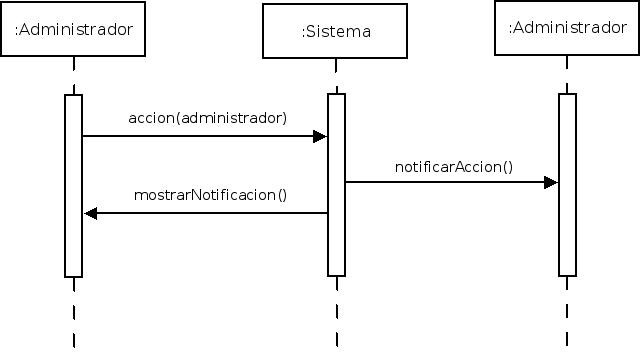
\includegraphics[scale=.50]{img/secuencias/gestion-administradores-activar-suspender.jpeg}
  \caption{Diagrama de secuencia: Gestión de administradores: Activar/Suspender administrador}
  \label{fig:secuencia-gestion-administradores-activar-suspender}
\end{figure}

\textbf{Contrato de operación: accion(administrador)}
\begin{itemize}
\item \textbf{Referencias cruzadas:} UC-26 (Cuadro \ref{tab:CU-activar-suspender-admin}).
\item \textbf{Responsabilidades:} El administrador podrá activar o suspender a otro administrador seleccionado.
\item \textbf{Precondiciones:} 
 \begin{itemize}
\item El administrador se ha identificado en el sistema previamente.
\item El administrador seleccionado debe estar activo para ser suspendido o viceversa.
\end {itemize}
\item \textbf{Postcondiciones:} 
 \begin{itemize}
\item Se realizará la acción seleccionada por el administrador \textit{(activar, suspender)} referente a otro administrador específico.
\end {itemize}
\end {itemize}

\textbf{Contrato de operación: notificarAccion()}
\begin{itemize}
\item \textbf{Referencias cruzadas:} UC-26 (Cuadro \ref{tab:CU-activar-suspender-admin}).
\item \textbf{Responsabilidades:} Mandar una notificación de suspensión/activación de la cuenta al administrador.
\item \textbf{Precondiciones:} 
 \begin{itemize}
\item Se ha suspendido/activado la cuenta de un administrador.
\end {itemize}
\item \textbf{Postcondiciones:} 
 \begin{itemize}
\item Se creará una nueva notificación de activación o suspensión de cuenta para el administrador seleccionado.
\end {itemize}
\end {itemize}

\textbf{Contrato de operación: mostrarNotificacion()}
\begin{itemize}
\item \textbf{Referencias cruzadas:} UC-26 (Cuadro \ref{tab:CU-activar-suspender-admin}).
\item \textbf{Responsabilidades:} Se mostrará un mensaje de acción por pantalla.
\item \textbf{Precondiciones:} 
 \begin{itemize}
\item Se ha realizado la acción correspondiente para activar el mensaje.
\end {itemize}
\item \textbf{Postcondiciones:} 
 \begin{itemize}
\item Se muestra el mensaje correspondiente a la acción en la pantalla, a modo de notificación para el administrador. Este puede ser confirmación de la acción o algún tipo de error en la ejecución de la misma.
\end {itemize}
\end {itemize}


\vspace{10mm}

\begin{figure}[H]
\centering
  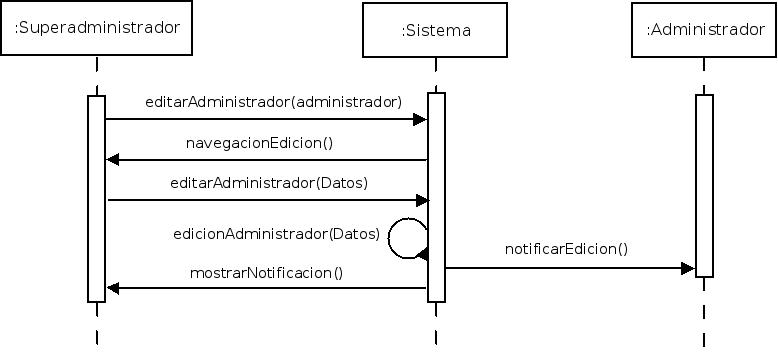
\includegraphics[scale=.50]{img/secuencias/gestion-administradores-editar-administrador.jpeg}
  \caption{Diagrama de secuencia: Gestión de administradores: Editar administrador}
  \label{fig:secuencia-gestion-administradores-editar-administrador}
\end{figure}

\textbf{Contrato de operación: editarAdministrador(administrador)}
\begin{itemize}
\item \textbf{Referencias cruzadas:} UC-27 (Cuadro \ref{tab:CU-editar-admin}).
\item \textbf{Responsabilidades:} Se informará al sistema de la acción de edición de un administrador específico por parte del superadministrador.
\item \textbf{Precondiciones:} 
 \begin{itemize}
\item El superadministrador se ha identificado en el sistema previamente.
\end {itemize}
\item \textbf{Postcondiciones:} 
 \begin{itemize}
\item Se manda la solicitud de edición del administrador seleccionado.
\end {itemize}
\end {itemize}

\textbf{Contrato de operación: navegacionEdicion()}
\begin{itemize}
\item \textbf{Referencias cruzadas:} UC-27 (Cuadro \ref{tab:CU-editar-admin}).
\item \textbf{Responsabilidades:} El sistema mostrará la página correspondiente a la edición de los datos del administrador.
\item \textbf{Precondiciones:} 
 \begin{itemize}
\item Se ha realizado la acción correspondiente para activar la navegación.
\end {itemize}
\item \textbf{Postcondiciones:} 
 \begin{itemize}
\item Se mostrará la página de edición del perfil del administrador seleccionado.
\end {itemize}
\end {itemize}

\textbf{Contrato de operación: editarAdministrador(Datos)}
\begin{itemize}
\item \textbf{Referencias cruzadas:} UC-27 (Cuadro \ref{tab:CU-editar-admin}).
\item \textbf{Responsabilidades:} Se mandará al sistema los datos del administrador para que este sea editado.
\item \textbf{Precondiciones:} 
 \begin{itemize}
\item El superadministrador se ha identificado en el sistema previamente.
\end {itemize}
\item \textbf{Postcondiciones:} 
 \begin{itemize}
\item Se envía el formulario de datos del administrador a editar al sistema.
\end {itemize}
\end {itemize}

\textbf{Contrato de operación: edicionAdministrador(Datos)}
\begin{itemize}
\item \textbf{Referencias cruzadas:} UC-27 (Cuadro \ref{tab:CU-editar-admin}).
\item \textbf{Responsabilidades:} Se realizará la edición de los datos del administrador, guardándolos en el sistema.
\item \textbf{Precondiciones:} 
 \begin{itemize}
\item Se ha enviado el formulario con los datos a editar.
\end {itemize}
\item \textbf{Postcondiciones:} 
 \begin{itemize}
\item El sistema guarda los datos recibidos para el administrador específico en la base de datos.
\end {itemize}
\end {itemize}

\textbf{Contrato de operación: notificarEdicion()}
\begin{itemize}
\item \textbf{Referencias cruzadas:} UC-27 (Cuadro \ref{tab:CU-editar-admin}).
\item \textbf{Responsabilidades:} Mandar una notificación de edición del perfil por parte del superadministrador al administrador.
\item \textbf{Precondiciones:} 
 \begin{itemize}
\item Se ha editado los datos del administrador por parte del superadministrador.
\end {itemize}
\item \textbf{Postcondiciones:} 
 \begin{itemize}
\item Se creará una nueva notificación de edición del perfil para el administrador seleccionado, indicando quién lo ha modificado.
\end {itemize}
\end {itemize}

\textbf{Contrato de operación: mostrarNotificacion()}
\begin{itemize}
\item \textbf{Referencias cruzadas:} UC-27 (Cuadro \ref{tab:CU-editar-admin}).
\item \textbf{Responsabilidades:} Se mostrará un mensaje de acción por pantalla.
\item \textbf{Precondiciones:} 
 \begin{itemize}
\item Se ha realizado la acción correspondiente para activar el mensaje.
\end {itemize}
\item \textbf{Postcondiciones:} 
 \begin{itemize}
\item Se muestra el mensaje correspondiente a la acción en la pantalla, a modo de notificación para el superadministrador. Este puede ser confirmación de la acción o algún tipo de error en la ejecución de la misma.
\end {itemize}
\end {itemize}


\vspace{10mm}

\begin{figure}[H]
\centering
  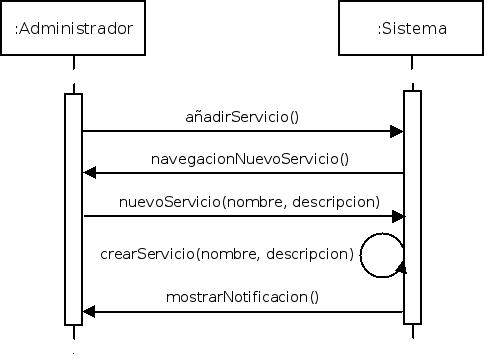
\includegraphics[scale=.55]{img/secuencias/gestion-servicios-alta-servicio.jpeg}
  \caption{Diagrama de secuencia: Gestión de servicios: Alta servicio}
  \label{fig:secuencia-gestion-servicios-alta-servicio}
\end{figure}

\textbf{Contrato de operación: añadirServicio()}
\begin{itemize}
\item \textbf{Referencias cruzadas:} UC-28 (Cuadro \ref{tab:CU-alta-servicio}).
\item \textbf{Responsabilidades:} Solicitar al sistema crear un nuevo servicio.
\item \textbf{Precondiciones:} 
 \begin{itemize}
\item El administrador se ha identificado en el sistema previamente.
\end {itemize}
\item \textbf{Postcondiciones:} 
 \begin{itemize}
\item Se enviará al sistema la solicitud de crear un nuevo servicio por parte del administrador.
\end {itemize}
\end {itemize}
\end{figure}

\textbf{Contrato de operación: navegacionNuevoServicio()}
\begin{itemize}
\item \textbf{Referencias cruzadas:} UC-28 (Cuadro \ref{tab:CU-alta-servicio}).
\item \textbf{Responsabilidades:} El sistema mostrará la ventana correspondiente a la creación de un nuevo servicio.
\item \textbf{Precondiciones:} 
 \begin{itemize}
\item Se ha realizado la acción correspondiente para activar la navegación.
\end {itemize}
\item \textbf{Postcondiciones:} 
 \begin{itemize}
\item Se mostrará la ventana de creación de un servicio nuevo en la interfaz del administrador.
\end {itemize}
\end {itemize}

\textbf{Contrato de operación: nuevoServicio(nombre, descripcion)}
\begin{itemize}
\item \textbf{Referencias cruzadas:} UC-28 (Cuadro \ref{tab:CU-alta-servicio}).
\item \textbf{Responsabilidades:} Se mandará al sistema los datos necesarios para la creación de un nuevo servicio.
\item \textbf{Precondiciones:} 
 \begin{itemize}
\item El administrador se ha identificado en el sistema previamente.
\end {itemize}
\item \textbf{Postcondiciones:} 
 \begin{itemize}
\item Se envía al sistema el nombre y la descripción del servicio a añadir.
\end {itemize}
\end {itemize}
\end{figure}

\textbf{Contrato de operación: crearServicio(nombre, descripcion)}
\begin{itemize}
\item \textbf{Referencias cruzadas:} UC-28 (Cuadro \ref{tab:CU-alta-servicio}).
\item \textbf{Responsabilidades:} Creación de un nuevo servicio con los datos recibidos.
\item \textbf{Precondiciones:} 
 \begin{itemize}
\item Se han recibido los datos de creación de un nuevo servicio.
\end {itemize}
\item \textbf{Postcondiciones:} 
 \begin{itemize}
 \item Se comprueban que el nombre del servicio es único.
\item Se crea un nuevo servicio y se introducen los datos en la base de datos.
\end {itemize}
\end {itemize}

\textbf{Contrato de operación: mostrarNotificacion()}
\begin{itemize}
\item \textbf{Referencias cruzadas:} UC-28 (Cuadro \ref{tab:CU-alta-servicio}).
\item \textbf{Responsabilidades:} Se mostrará un mensaje de acción por pantalla.
\item \textbf{Precondiciones:} 
 \begin{itemize}
\item Se ha realizado la acción correspondiente para activar el mensaje.
\end {itemize}
\item \textbf{Postcondiciones:} 
 \begin{itemize}
\item Se muestra el mensaje correspondiente a la acción en la pantalla, a modo de notificación para el administrador. Este puede ser confirmación de la acción o algún tipo de error en la ejecución de la misma.
\end {itemize}
\end {itemize}


\vspace{10mm}

\begin{figure}[H]
\centering
  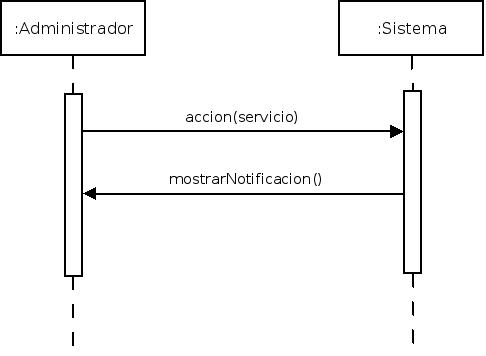
\includegraphics[scale=.55]{img/secuencias/gestion-servicios-suspender-activar-servicio.jpeg}
  \caption{Diagrama de secuencia: Gestión de servicios: Activar/Suspender servicio}
  \label{fig:secuencia-gestion-servicios-suspender-activar-servicio}
\end{figure}

\textbf{Contrato de operación: accion(servicio)}
\begin{itemize}
\item \textbf{Referencias cruzadas:} UC-29 (Cuadro \ref{tab:CU-activar-suspender-servicio}).
\item \textbf{Responsabilidades:} El administrador podrá activar o suspender el servicio seleccionado.
\item \textbf{Precondiciones:} 
 \begin{itemize}
\item El administrador se ha identificado en el sistema previamente.
\item El servicio seleccionado debe estar activo para ser suspendido o viceversa.
\end {itemize}
\item \textbf{Postcondiciones:} 
 \begin{itemize}
\item Se realizará la acción seleccionada por el administrador \textit{(activar, suspender)} referente a un servicio específico.
\end {itemize}
\end {itemize}

\textbf{Contrato de operación: mostrarNotificacion()}
\begin{itemize}
\item \textbf{Referencias cruzadas:} UC-29 (Cuadro \ref{tab:CU-activar-suspender-servicio}).
\item \textbf{Responsabilidades:} Se mostrará un mensaje de acción por pantalla.
\item \textbf{Precondiciones:} 
 \begin{itemize}
\item Se ha realizado la acción correspondiente para activar el mensaje.
\end {itemize}
\item \textbf{Postcondiciones:} 
 \begin{itemize}
\item Se muestra el mensaje correspondiente a la acción en la pantalla, a modo de notificación para el administrador. Este puede ser confirmación de la acción o algún tipo de error en la ejecución de la misma.
\end {itemize}
\end {itemize}


\vspace{10mm}

\begin{figure}[H]
\centering
  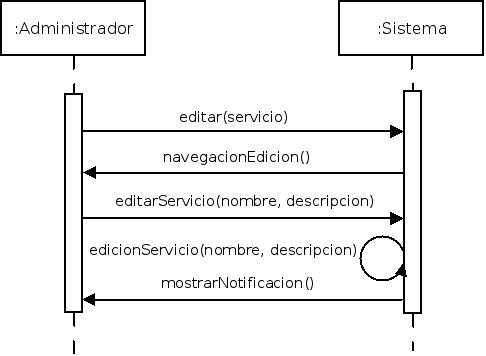
\includegraphics[scale=.55]{img/secuencias/gestion-servicios-editar-servicio.jpeg}
  \caption{Diagrama de secuencia: Gestión de servicios: Editar servicio}
  \label{fig:secuencia-gestion-servicios-editar-servicio}
\end{figure}

\textbf{Contrato de operación: editar(servicio)}
\begin{itemize}
\item \textbf{Referencias cruzadas:} UC-30 (Cuadro \ref{tab:CU-editar-servicio}).
\item \textbf{Responsabilidades:} Se solicitará al sistema la edición de un servicio específico por parte del administrador.
\item \textbf{Precondiciones:} 
 \begin{itemize}
\item El administrador se ha identificado en el sistema previamente.
\end {itemize}
\item \textbf{Postcondiciones:} 
 \begin{itemize}
\item Se manda la solicitud de edición del servicio seleccionado.
\end {itemize}
\end {itemize}

\textbf{Contrato de operación: navegacionEdicion()}
\begin{itemize}
\item \textbf{Referencias cruzadas:} UC-30 (Cuadro \ref{tab:CU-editar-servicio}).
\item \textbf{Responsabilidades:} El sistema mostrará la página correspondiente a la edición del servicio.
\item \textbf{Precondiciones:} 
 \begin{itemize}
\item Se ha realizado la acción correspondiente para activar la navegación.
\end {itemize}
\item \textbf{Postcondiciones:} 
 \begin{itemize}
\item Se mostrará la ventana de edición del servicio seleccionado.
\end {itemize}
\end {itemize}

\textbf{Contrato de operación: editarServicio(nombre, descripcion)}
\begin{itemize}
\item \textbf{Referencias cruzadas:} UC-30 (Cuadro \ref{tab:CU-editar-servicio}).
\item \textbf{Responsabilidades:} Se mandará al sistema los datos del servicio para que este sea editado.
\item \textbf{Precondiciones:} 
 \begin{itemize}
\item El administrador se ha identificado en el sistema previamente.
\end {itemize}
\item \textbf{Postcondiciones:} 
 \begin{itemize}
\item Se envía el nombre y la descripción del servicio a editar al sistema.
\end {itemize}
\end {itemize}

\textbf{Contrato de operación: edicionServicio(nombre, descripcion)}
\begin{itemize}
\item \textbf{Referencias cruzadas:} UC-30 (Cuadro \ref{tab:CU-editar-servicio}).
\item \textbf{Responsabilidades:} Se realizará la edición de los datos del servicio, guardándolos en el sistema.
\item \textbf{Precondiciones:} 
 \begin{itemize}
\item Se ha enviado el formulario con los datos a editar.
\end {itemize}
\item \textbf{Postcondiciones:} 
 \begin{itemize}
 \item Se comprueba que el nombre del servicio sea único.
\item El sistema guarda los datos recibidos para el servicio específico en la base de datos.
\end {itemize}
\end {itemize}

\textbf{Contrato de operación: mostrarNotificacion()}
\begin{itemize}
\item \textbf{Referencias cruzadas:} UC-30 (Cuadro \ref{tab:CU-editar-servicio}).
\item \textbf{Responsabilidades:} Se mostrará un mensaje de acción por pantalla.
\item \textbf{Precondiciones:} 
 \begin{itemize}
\item Se ha realizado la acción correspondiente para activar el mensaje.
\end {itemize}
\item \textbf{Postcondiciones:} 
 \begin{itemize}
\item Se muestra el mensaje correspondiente a la acción en la pantalla, a modo de notificación para el administrador. Este puede ser confirmación de la acción o algún tipo de error en la ejecución de la misma.
\end {itemize}
\end {itemize}


\vspace{10mm}

\begin{figure}[H]
\centering
  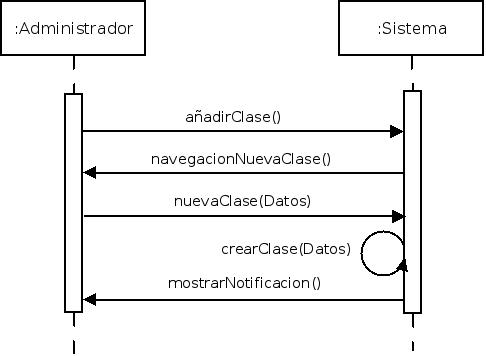
\includegraphics[scale=.55]{img/secuencias/gestion-servicios-alta-clase.jpeg}
  \caption{Diagrama de secuencia: Gestión de servicios: Alta clase}
  \label{fig:secuencia-gestion-servicios-alta-clase}
\end{figure}

\textbf{Contrato de operación: añadirClase()}
\begin{itemize}
\item \textbf{Referencias cruzadas:} UC-31 (Cuadro \ref{tab:CU-alta-clase}).
\item \textbf{Responsabilidades:} Solicitar al sistema crear una nueva clase.
\item \textbf{Precondiciones:} 
 \begin{itemize}
\item El administrador se ha identificado en el sistema previamente.
\end {itemize}
\item \textbf{Postcondiciones:} 
 \begin{itemize}
\item Se enviará al sistema la solicitud de crear una nueva clase por parte del administrador.
\end {itemize}
\end {itemize}
\end{figure}

\textbf{Contrato de operación: navegacionNuevaClase()}
\begin{itemize}
\item \textbf{Referencias cruzadas:} UC-31 (Cuadro \ref{tab:CU-alta-clase}).
\item \textbf{Responsabilidades:} El sistema mostrará la ventana correspondiente a la creación de una nueva clase.
\item \textbf{Precondiciones:} 
 \begin{itemize}
\item Se ha realizado la acción correspondiente para activar la navegación.
\end {itemize}
\item \textbf{Postcondiciones:} 
 \begin{itemize}
\item Se mostrará la ventana de creación de una clase nueva en la interfaz del administrador.
\end {itemize}
\end {itemize}

\textbf{Contrato de operación: nuevaClase(Datos)}
\begin{itemize}
\item \textbf{Referencias cruzadas:} UC-31 (Cuadro \ref{tab:CU-alta-clase}).
\item \textbf{Responsabilidades:} Se mandará al sistema los datos necesarios para la creación de una nueva clase.
\item \textbf{Precondiciones:} 
 \begin{itemize}
\item El administrador se ha identificado en el sistema previamente.
\end {itemize}
\item \textbf{Postcondiciones:} 
 \begin{itemize}
\item Se envía al sistema los datos de la clase a añadir.
\end {itemize}
\end {itemize}
\end{figure}

\textbf{Contrato de operación: crearClase(Datos)}
\begin{itemize}
\item \textbf{Referencias cruzadas:} UC-31 (Cuadro \ref{tab:CU-alta-clase}).
\item \textbf{Responsabilidades:} Creación de una nueva clase con los datos recibidos.
\item \textbf{Precondiciones:} 
 \begin{itemize}
\item Se han recibido los datos de creación de una nueva clase.
\end {itemize}
\item \textbf{Postcondiciones:} 
 \begin{itemize}
 \item Se comprueban que los datos recibidos son correctos.
\item Se crea una nueva clase y se introducen los datos en la base de datos.
\end {itemize}
\end {itemize}

\textbf{Contrato de operación: mostrarNotificacion()}
\begin{itemize}
\item \textbf{Referencias cruzadas:} UC-31 (Cuadro \ref{tab:CU-alta-clase}).
\item \textbf{Responsabilidades:} Se mostrará un mensaje de acción por pantalla.
\item \textbf{Precondiciones:} 
 \begin{itemize}
\item Se ha realizado la acción correspondiente para activar el mensaje.
\end {itemize}
\item \textbf{Postcondiciones:} 
 \begin{itemize}
\item Se muestra el mensaje correspondiente a la acción en la pantalla, a modo de notificación para el administrador. Este puede ser confirmación de la acción o algún tipo de error en la ejecución de la misma.
\end {itemize}
\end {itemize}


\vspace{10mm}

\begin{figure}[H]
\centering
  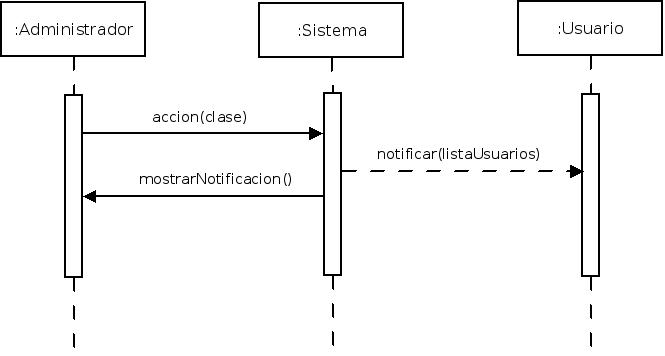
\includegraphics[scale=.55]{img/secuencias/gestion-servicios-suspender-activar-clase.jpeg}
  \caption{Diagrama de secuencia: Gestión de servicios: Activar/Suspender clase}
  \label{fig:secuencia-gestion-servicios-suspender-activar-clase}
\end{figure}

\textbf{Contrato de operación: accion(clase)}
\begin{itemize}
\item \textbf{Referencias cruzadas:} UC-32 (Cuadro \ref{tab:CU-activar-suspender-clase}).
\item \textbf{Responsabilidades:} El administrador podrá activar o suspender la clase seleccionada.
\item \textbf{Precondiciones:} 
 \begin{itemize}
\item El administrador se ha identificado en el sistema previamente.
\item La clase seleccionada debe estar activa para ser suspendida o viceversa.
\end {itemize}
\item \textbf{Postcondiciones:} 
 \begin{itemize}
\item Se realizará la acción seleccionada por el administrador \textit{(activar, suspender)} referente a una clase específica.
\end {itemize}
\end {itemize}

\textbf{Contrato de operación: notificar(listaUsuarios)}
\begin{itemize}
\item \textbf{Referencias cruzadas:} UC-32 (Cuadro \ref{tab:CU-activar-suspender-clase}).
\item \textbf{Responsabilidades:} Mandar una notificación de activación o suspensión de una clase específica por parte del administrador a todos los usuarios con reserva en la misma, en caso que existan.
\item \textbf{Precondiciones:} 
 \begin{itemize}
\item Se ha activado o suspendido una clase.
\end {itemize}
\item \textbf{Postcondiciones:} 
 \begin{itemize}
\item Se creará una nueva notificación de activación o suspensión de una determinada clase para cada uno de los usuarios con reserva en la misma.
\end {itemize}
\end {itemize}

\textbf{Contrato de operación: mostrarNotificacion()}
\begin{itemize}
\item \textbf{Referencias cruzadas:} UC-32 (Cuadro \ref{tab:CU-activar-suspender-clase}).
\item \textbf{Responsabilidades:} Se mostrará un mensaje de acción por pantalla.
\item \textbf{Precondiciones:} 
 \begin{itemize}
\item Se ha realizado la acción correspondiente para activar el mensaje.
\end {itemize}
\item \textbf{Postcondiciones:} 
 \begin{itemize}
\item Se muestra el mensaje correspondiente a la acción en la pantalla, a modo de notificación para el administrador. Este puede ser confirmación de la acción o algún tipo de error en la ejecución de la misma.
\end {itemize}
\end {itemize}


\vspace{10mm}

\begin{figure}[H]
\centering
  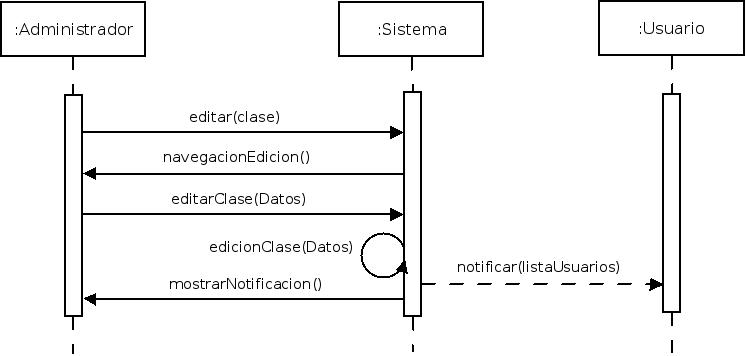
\includegraphics[scale=.50]{img/secuencias/gestion-servicios-editar-clase.jpeg}
  \caption{Diagrama de secuencia: Gestión de servicios: Editar clase}
  \label{fig:secuencia-editar-clase}
\end{figure}

\textbf{Contrato de operación: editar(clase)}
\begin{itemize}
\item \textbf{Referencias cruzadas:} UC-33 (Cuadro \ref{tab:CU-editar-clase}).
\item \textbf{Responsabilidades:} Se solicitará al sistema la edición de una clase específica por parte del administrador.
\item \textbf{Precondiciones:} 
 \begin{itemize}
\item El administrador se ha identificado en el sistema previamente.
\end {itemize}
\item \textbf{Postcondiciones:} 
 \begin{itemize}
\item Se manda la solicitud de edición de la clase seleccionada.
\end {itemize}
\end {itemize}

\textbf{Contrato de operación: navegacionEdicion()}
\begin{itemize}
\item \textbf{Referencias cruzadas:} UC-33 (Cuadro \ref{tab:CU-editar-clase}).
\item \textbf{Responsabilidades:} El sistema mostrará la página correspondiente a la edición de la clase.
\item \textbf{Precondiciones:} 
 \begin{itemize}
\item Se ha realizado la acción correspondiente para activar la navegación.
\end {itemize}
\item \textbf{Postcondiciones:} 
 \begin{itemize}
\item Se mostrará la ventana de edición de la clase seleccionada.
\end {itemize}
\end {itemize}

\textbf{Contrato de operación: editarClase(Datos)}
\begin{itemize}
\item \textbf{Referencias cruzadas:} UC-33 (Cuadro \ref{tab:CU-editar-clase}).
\item \textbf{Responsabilidades:} Se mandará al sistema los datos de la clase para que esta sea editada.
\item \textbf{Precondiciones:} 
 \begin{itemize}
\item El administrador se ha identificado en el sistema previamente.
\end {itemize}
\item \textbf{Postcondiciones:} 
 \begin{itemize}
\item Se envían todos los datos del formulario de edición de la clase al sistema.
\end {itemize}
\end {itemize}

\textbf{Contrato de operación: edicionClase(Datos)}
\begin{itemize}
\item \textbf{Referencias cruzadas:} UC-33 (Cuadro \ref{tab:CU-editar-clase}).
\item \textbf{Responsabilidades:} Se realizará la edición de los datos de la clase, guardándolos en el sistema.
\item \textbf{Precondiciones:} 
 \begin{itemize}
\item Se ha enviado el formulario con los datos a editar.
\end {itemize}
\item \textbf{Postcondiciones:} 
 \begin{itemize}
 \item Se comprueban que los datos recibidos son correctos.
\item El sistema guarda los datos recibidos para la clase específica en la base de datos.
\end {itemize}
\end {itemize}

\textbf{Contrato de operación: mostrarNotificacion()}
\begin{itemize}
\item \textbf{Referencias cruzadas:} UC-33 (Cuadro \ref{tab:CU-editar-clase}).
\item \textbf{Responsabilidades:} Se mostrará un mensaje de acción por pantalla.
\item \textbf{Precondiciones:} 
 \begin{itemize}
\item Se ha realizado la acción correspondiente para activar el mensaje.
\end {itemize}
\item \textbf{Postcondiciones:} 
 \begin{itemize}
\item Se muestra el mensaje correspondiente a la acción en la pantalla, a modo de notificación para el administrador. Este puede ser confirmación de la acción o algún tipo de error en la ejecución de la misma.
\end {itemize}
\end {itemize}


\vspace{10mm}

\begin{figure}[H]
\centering
  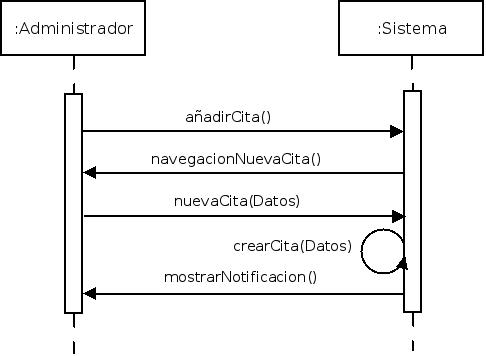
\includegraphics[scale=.55]{img/secuencias/gestion-servicios-alta-cita.jpeg}
  \caption{Diagrama de secuencia: Gestión de servicios: Alta cita}
  \label{fig:secuencia-gestion-servicios-alta-cita}
\end{figure}

\textbf{Contrato de operación: añadirCita()}
\begin{itemize}
\item \textbf{Referencias cruzadas:} UC-34 (Cuadro \ref{tab:CU-alta-cita}).
\item \textbf{Responsabilidades:} Solicitar al sistema crear una nueva cita.
\item \textbf{Precondiciones:} 
 \begin{itemize}
\item El administrador se ha identificado en el sistema previamente.
\end {itemize}
\item \textbf{Postcondiciones:} 
 \begin{itemize}
\item Se enviará al sistema la solicitud de crear una nueva cita por parte del administrador.
\end {itemize}
\end {itemize}
\end{figure}

\textbf{Contrato de operación: navegacionNuevaCita()}
\begin{itemize}
\item \textbf{Referencias cruzadas:} UC-34 (Cuadro \ref{tab:CU-alta-cita}).
\item \textbf{Responsabilidades:} El sistema mostrará la ventana correspondiente a la creación de una nueva cita.
\item \textbf{Precondiciones:} 
 \begin{itemize}
\item Se ha realizado la acción correspondiente para activar la navegación.
\end {itemize}
\item \textbf{Postcondiciones:} 
 \begin{itemize}
\item Se mostrará la ventana de creación de una cita nueva en la interfaz del administrador.
\end {itemize}
\end {itemize}

\textbf{Contrato de operación: nuevaCita(Datos)}
\begin{itemize}
\item \textbf{Referencias cruzadas:} UC-34 (Cuadro \ref{tab:CU-alta-cita}).
\item \textbf{Responsabilidades:} Se mandará al sistema los datos necesarios para la creación de una nueva cita.
\item \textbf{Precondiciones:} 
 \begin{itemize}
\item El administrador se ha identificado en el sistema previamente.
\end {itemize}
\item \textbf{Postcondiciones:} 
 \begin{itemize}
\item Se envía al sistema los datos de la cita a añadir.
\end {itemize}
\end {itemize}
\end{figure}

\textbf{Contrato de operación: crearCita(Datos)}
\begin{itemize}
\item \textbf{Referencias cruzadas:} UC-34 (Cuadro \ref{tab:CU-alta-cita}).
\item \textbf{Responsabilidades:} Creación de una nueva cita con los datos recibidos.
\item \textbf{Precondiciones:} 
 \begin{itemize}
\item Se han recibido los datos de creación de una nueva cita.
\end {itemize}
\item \textbf{Postcondiciones:} 
 \begin{itemize}
 \item Se comprueban que los datos recibidos son correctos.
\item Se crea una nueva cita y se introducen los datos en la base de datos.
\end {itemize}
\end {itemize}

\textbf{Contrato de operación: mostrarNotificacion()}
\begin{itemize}
\item \textbf{Referencias cruzadas:} UC-34 (Cuadro \ref{tab:CU-alta-cita}).
\item \textbf{Responsabilidades:} Se mostrará un mensaje de acción por pantalla.
\item \textbf{Precondiciones:} 
 \begin{itemize}
\item Se ha realizado la acción correspondiente para activar el mensaje.
\end {itemize}
\item \textbf{Postcondiciones:} 
 \begin{itemize}
\item Se muestra el mensaje correspondiente a la acción en la pantalla, a modo de notificación para el administrador. Este puede ser confirmación de la acción o algún tipo de error en la ejecución de la misma.
\end {itemize}
\end {itemize}


\vspace{10mm}

\begin{figure}[H]
\centering
  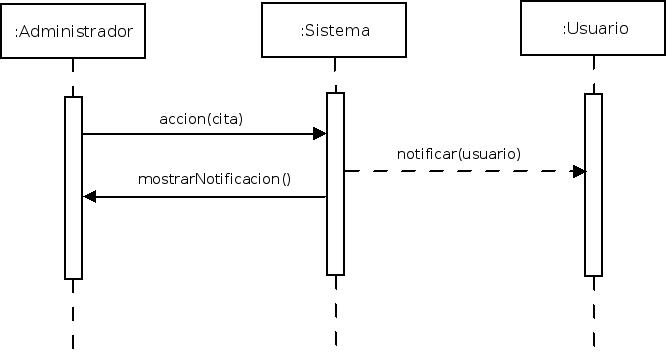
\includegraphics[scale=.55]{img/secuencias/gestion-servicios-suspender-activar-cita.jpeg}
  \caption{Diagrama de secuencia: Gestión de servicios: Activar/Suspender cita}
  \label{fig:secuencia-gestion-servicios-suspender-activar-cita}
\end{figure}

\textbf{Contrato de operación: accion(cita)}
\begin{itemize}
\item \textbf{Referencias cruzadas:} UC-35 (Cuadro \ref{tab:CU-activar-suspender-cita}).
\item \textbf{Responsabilidades:} El administrador podrá activar o suspender la cita seleccionada.
\item \textbf{Precondiciones:} 
 \begin{itemize}
\item El administrador se ha identificado en el sistema previamente.
\item La cita seleccionada debe estar activa para ser suspendida o viceversa.
\end {itemize}
\item \textbf{Postcondiciones:} 
 \begin{itemize}
\item Se realizará la acción seleccionada por el administrador \textit{(activar, suspender)} referente a una cita específica.
\end {itemize}
\end {itemize}

\textbf{Contrato de operación: notificar(listaUsuarios)}
\begin{itemize}
\item \textbf{Referencias cruzadas:} UC-35 (Cuadro \ref{tab:CU-activar-suspender-cita}).
\item \textbf{Responsabilidades:} Mandar una notificación de activación o suspensión de una cita específica por parte del administrador a todos los usuarios con reserva en la misma, en caso que existan.
\item \textbf{Precondiciones:} 
 \begin{itemize}
\item Se ha activado o suspendido una cita.
\end {itemize}
\item \textbf{Postcondiciones:} 
 \begin{itemize}
\item Se creará una nueva notificación de activación o suspensión de una determinada cita para cada uno de los usuarios con reserva en la misma.
\end {itemize}
\end {itemize}

\textbf{Contrato de operación: mostrarNotificacion()}
\begin{itemize}
\item \textbf{Referencias cruzadas:} UC-35 (Cuadro \ref{tab:CU-activar-suspender-cita}).
\item \textbf{Responsabilidades:} Se mostrará un mensaje de acción por pantalla.
\item \textbf{Precondiciones:} 
 \begin{itemize}
\item Se ha realizado la acción correspondiente para activar el mensaje.
\end {itemize}
\item \textbf{Postcondiciones:} 
 \begin{itemize}
\item Se muestra el mensaje correspondiente a la acción en la pantalla, a modo de notificación para el administrador. Este puede ser confirmación de la acción o algún tipo de error en la ejecución de la misma.
\end {itemize}
\end {itemize}


\vspace{10mm}

\begin{figure}[H]
\centering
  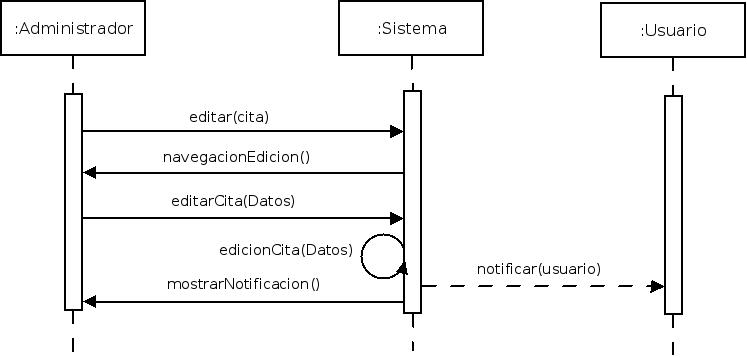
\includegraphics[scale=.50]{img/secuencias/gestion-servicios-editar-cita.jpeg}
  \caption{Diagrama de secuencia: Gestión de servicios: Editar cita}
  \label{fig:secuencia-gestion-servicios-editar-cita}
\end{figure}

\textbf{Contrato de operación: editar(cita)}
\begin{itemize}
\item \textbf{Referencias cruzadas:} UC-36 (Cuadro \ref{tab:CU-editar-cita}).
\item \textbf{Responsabilidades:} Se solicitará al sistema la edición de una cita específica por parte del administrador.
\item \textbf{Precondiciones:} 
 \begin{itemize}
\item El administrador se ha identificado en el sistema previamente.
\end {itemize}
\item \textbf{Postcondiciones:} 
 \begin{itemize}
\item Se manda la solicitud de edición de la cita seleccionada.
\end {itemize}
\end {itemize}

\textbf{Contrato de operación: navegacionEdicion()}
\begin{itemize}
\item \textbf{Referencias cruzadas:} UC-36 (Cuadro \ref{tab:CU-editar-cita}).
\item \textbf{Responsabilidades:} El sistema mostrará la página correspondiente a la edición de la cita.
\item \textbf{Precondiciones:} 
 \begin{itemize}
\item Se ha realizado la acción correspondiente para activar la navegación.
\end {itemize}
\item \textbf{Postcondiciones:} 
 \begin{itemize}
\item Se mostrará la ventana de edición de la cita seleccionada.
\end {itemize}
\end {itemize}

\textbf{Contrato de operación: editarCita(Datos)}
\begin{itemize}
\item \textbf{Referencias cruzadas:} UC-36 (Cuadro \ref{tab:CU-editar-cita}).
\item \textbf{Responsabilidades:} Se mandará al sistema los datos de la cita para que esta sea editada.
\item \textbf{Precondiciones:} 
 \begin{itemize}
\item El administrador se ha identificado en el sistema previamente.
\end {itemize}
\item \textbf{Postcondiciones:} 
 \begin{itemize}
\item Se envían todos los datos del formulario de edición de la cita al sistema.
\end {itemize}
\end {itemize}

\textbf{Contrato de operación: edicionCita(Datos)}
\begin{itemize}
\item \textbf{Referencias cruzadas:} UC-36 (Cuadro \ref{tab:CU-editar-cita}).
\item \textbf{Responsabilidades:} Se realizará la edición de los datos de la cita, guardándolos en el sistema.
\item \textbf{Precondiciones:} 
 \begin{itemize}
\item Se ha enviado el formulario con los datos a editar.
\end {itemize}
\item \textbf{Postcondiciones:} 
 \begin{itemize}
 \item Se comprueban que los datos recibidos son correctos.
\item El sistema guarda los datos recibidos para la cita específica en la base de datos.
\end {itemize}
\end {itemize}

\textbf{Contrato de operación: mostrarNotificacion()}
\begin{itemize}
\item \textbf{Referencias cruzadas:} UC-36 (Cuadro \ref{tab:CU-editar-cita}).
\item \textbf{Responsabilidades:} Se mostrará un mensaje de acción por pantalla.
\item \textbf{Precondiciones:} 
 \begin{itemize}
\item Se ha realizado la acción correspondiente para activar el mensaje.
\end {itemize}
\item \textbf{Postcondiciones:} 
 \begin{itemize}
\item Se muestra el mensaje correspondiente a la acción en la pantalla, a modo de notificación para el administrador. Este puede ser confirmación de la acción o algún tipo de error en la ejecución de la misma.
\end {itemize}
\end {itemize}


\vspace{10mm}

\begin{figure}[H]
\centering
  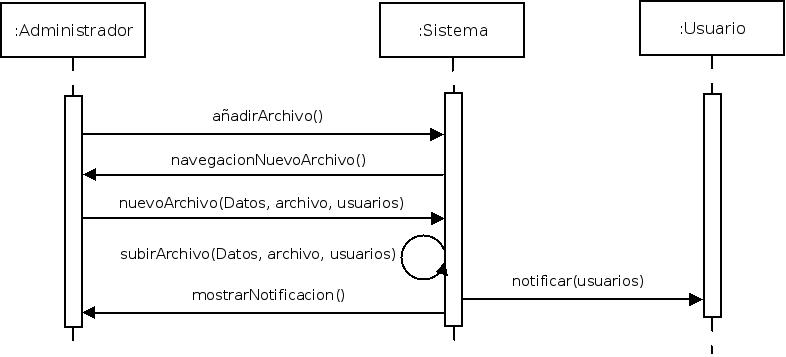
\includegraphics[scale=.50]{img/secuencias/gestion-servicios-subir-archivo.jpeg}
  \caption{Diagrama de secuencia: Gestión de servicios: Subir archivo}
  \label{fig:secuencia-gestion-servicios-subir-archivo}
\end{figure}

\textbf{Contrato de operación: añadirArchivo()}
\begin{itemize}
\item \textbf{Referencias cruzadas:} UC-37 (Cuadro \ref{tab:CU-subir-archivo}).
\item \textbf{Responsabilidades:} Solicitar al sistema subir un archivo.
\item \textbf{Precondiciones:} 
 \begin{itemize}
\item El administrador se ha identificado en el sistema previamente.
\end {itemize}
\item \textbf{Postcondiciones:} 
 \begin{itemize}
\item Se enviará al sistema la solicitud de subir un documento por parte del administrador.
\end {itemize}
\end {itemize}
\end{figure}

\textbf{Contrato de operación: navegacionNuevoArchivo()}
\begin{itemize}
\item \textbf{Referencias cruzadas:} UC-37 (Cuadro \ref{tab:CU-subir-archivo}).
\item \textbf{Responsabilidades:} El sistema mostrará la ventana correspondiente a la subida de un nuevo archivo.
\item \textbf{Precondiciones:} 
 \begin{itemize}
\item Se ha realizado la acción correspondiente para activar la navegación.
\end {itemize}
\item \textbf{Postcondiciones:} 
 \begin{itemize}
\item Se mostrará la ventana de subida de un nuevo archivo en la interfaz del administrador.
\end {itemize}
\end {itemize}

\textbf{Contrato de operación: nuevoArchivo(Datos, archivo, usuarios)}
\begin{itemize}
\item \textbf{Referencias cruzadas:} UC-37 (Cuadro \ref{tab:CU-subir-archivo}).
\item \textbf{Responsabilidades:} Se mandará al sistema los datos necesarios para subir el archivo.
\item \textbf{Precondiciones:} 
 \begin{itemize}
\item El administrador se ha identificado en el sistema previamente.
\end {itemize}
\item \textbf{Postcondiciones:} 
 \begin{itemize}
\item Se envía al sistema los datos del archivo a subir, el propio archivo y el usuario o lista de usuarios a los que el documento va destinado.
\end {itemize}
\end {itemize}
\end{figure}

\textbf{Contrato de operación: subirArchivo(Datos, archivo, usuarios)}
\begin{itemize}
\item \textbf{Referencias cruzadas:} UC-37 (Cuadro \ref{tab:CU-subir-archivo}).
\item \textbf{Responsabilidades:} Almacenamiento de una nuevo archivo, con los datos y archivo recibidos.
\item \textbf{Precondiciones:} 
 \begin{itemize}
\item Se han recibido los datos y el archivo para la creación de un documento nuevo.
\end {itemize}
\item \textbf{Postcondiciones:} 
 \begin{itemize}
 \item Se comprueban que los datos recibidos y el archivo son correctos.
\item Se crea y almacena un nuevo archivo y se introducen los datos en la base de datos.
\item Se especifica qué usuarios tienen acceso al archivo para su posterior consulta o descarga.
\end {itemize}
\end {itemize}

\textbf{Contrato de operación: notificar(usuarios)}
\begin{itemize}
\item \textbf{Referencias cruzadas:} UC-37 (Cuadro \ref{tab:CU-subir-archivo}).
\item \textbf{Responsabilidades:} Mandar una notificación de documento disponible a los usuarios especificados al subir el archivo, en caso que existan.
\item \textbf{Precondiciones:} 
 \begin{itemize}
\item Se ha subido al sistema un nuevo documento.
\end {itemize}
\item \textbf{Postcondiciones:} 
 \begin{itemize}
\item Se creará una nueva notificación de archivo subido disponible para cada uno de los usuarios especificados por el administrador en el proceso de subida.
\end {itemize}
\end {itemize}

\textbf{Contrato de operación: mostrarNotificacion()}
\begin{itemize}
\item \textbf{Referencias cruzadas:} UC-37 (Cuadro \ref{tab:CU-subir-archivo}).
\item \textbf{Responsabilidades:} Se mostrará un mensaje de acción por pantalla.
\item \textbf{Precondiciones:} 
 \begin{itemize}
\item Se ha realizado la acción correspondiente para activar el mensaje.
\end {itemize}
\item \textbf{Postcondiciones:} 
 \begin{itemize}
\item Se muestra el mensaje correspondiente a la acción en la pantalla, a modo de notificación para el administrador. Este puede ser confirmación de la acción o algún tipo de error en la ejecución de la misma.
\end {itemize}
\end {itemize}


\vspace{10mm}

\begin{figure}[H]
\centering
  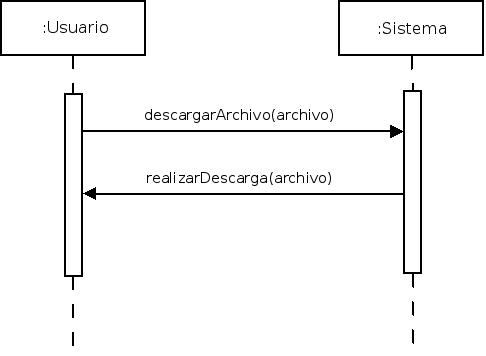
\includegraphics[scale=.55]{img/secuencias/gestion-servicios-descargar-archivo.jpeg}
  \caption{Diagrama de secuencia: Gestión de servicios: Descargar archivo}
  \label{fig:secuencia-gestion-servicios-descargar-archivo}
\end{figure}

\textbf{Contrato de operación: descargarArchivo(archivo)}
\begin{itemize}
\item \textbf{Referencias cruzadas:} UC-38 (Cuadro \ref{tab:CU-descargar-archivo}).
\item \textbf{Responsabilidades:} Solicitar al sistema la descarga del archivo seleccionado.
\item \textbf{Precondiciones:} 
 \begin{itemize}
\item El usuario se ha identificado en el sistema previamente.
\item Existen documentos subidos destinados al usuario.
\end {itemize}
\item \textbf{Postcondiciones:} 
 \begin{itemize}
\item El usuario manda al sistema la solicitud de descarga de un archivo específico.
\end {itemize}
\end {itemize}

\textbf{Contrato de operación: realizarDescarga(archivo)}
\begin{itemize}
\item \textbf{Referencias cruzadas:} UC-38 (Cuadro \ref{tab:CU-descargar-archivo}).
\item \textbf{Responsabilidades:} Realizar la descarga del documento seleccionado al dispositivo del usuario.
\item \textbf{Precondiciones:} 
 \begin{itemize}
\item El usuario ha solicitado la descarga de un archivo específico.
\end {itemize}
\item \textbf{Postcondiciones:} 
 \begin{itemize}
\item El documento seleccionado se descargará al dispositivo del usuario.
\end {itemize}
\end {itemize}


\vspace{10mm}

\begin{figure}[H]
\centering
  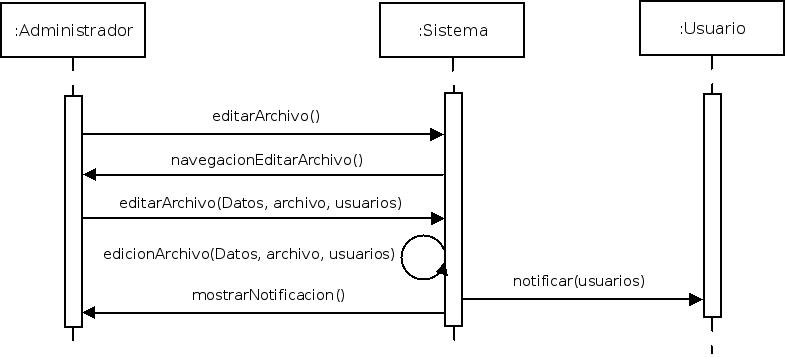
\includegraphics[scale=.50]{img/secuencias/gestion-servicios-editar-archivo.jpeg}
  \caption{Diagrama de secuencia: Gestión de servicios: Editar archivo}
  \label{fig:secuencia-gestion-servicios-editar-archivo}
\end{figure}

\textbf{Contrato de operación: editar(archivo)}
\begin{itemize}
\item \textbf{Referencias cruzadas:} UC-39 (Cuadro \ref{tab:CU-editar-archivo}).
\item \textbf{Responsabilidades:} Se solicitará al sistema la edición de un archivo específico por parte del administrador.
\item \textbf{Precondiciones:} 
 \begin{itemize}
\item El administrador se ha identificado en el sistema previamente.
\item Existen documentos subidos.
\end {itemize}
\item \textbf{Postcondiciones:} 
 \begin{itemize}
\item Se manda la solicitud de edición del archivo seleccionado.
\end {itemize}
\end {itemize}

\textbf{Contrato de operación: navegacionEdicion()}
\begin{itemize}
\item \textbf{Referencias cruzadas:} UC-39 (Cuadro \ref{tab:CU-editar-archivo}).
\item \textbf{Responsabilidades:} El sistema mostrará la página correspondiente a la edición del archivo.
\item \textbf{Precondiciones:} 
 \begin{itemize}
\item Se ha realizado la acción correspondiente para activar la navegación.
\end {itemize}
\item \textbf{Postcondiciones:} 
 \begin{itemize}
\item Se mostrará la ventana de edición del archivo seleccionado.
\end {itemize}
\end {itemize}

\textbf{Contrato de operación: editarArchivo(Datos, usuarios)}
\begin{itemize}
\item \textbf{Referencias cruzadas:} UC-39 (Cuadro \ref{tab:CU-editar-archivo}).
\item \textbf{Responsabilidades:} Se mandará al sistema los datos del archivo y usuarios a los que va destinado para que sea editado.
\item \textbf{Precondiciones:} 
 \begin{itemize}
\item El administrador se ha identificado en el sistema previamente.
\end {itemize}
\item \textbf{Postcondiciones:} 
 \begin{itemize}
\item Se envían todos los datos del formulario de edición del archivo al sistema.
\item Se especifican todos los usuarios que tendrán acceso al documento.
\end {itemize}
\end {itemize}

\textbf{Contrato de operación: edicionArchivo(Datos)}
\begin{itemize}
\item \textbf{Referencias cruzadas:} UC-39 (Cuadro \ref{tab:CU-editar-archivo}).
\item \textbf{Responsabilidades:} Se realizará la edición de los datos del archivo y la lista de usuarios con permiso para su acceso, guardándolos en el sistema.
\item \textbf{Precondiciones:} 
 \begin{itemize}
\item Se ha enviado el formulario con los datos a editar y la lista de usuarios a los que el documento va destinado.
\end {itemize}
\item \textbf{Postcondiciones:} 
 \begin{itemize}
 \item Se comprueban que los datos recibidos son correctos.
\item El sistema guarda los datos recibidos para el archivo específico en la base de datos.
\item El sistema da autorización a los usuarios especificados para que tengan acceso al archivo.
\end {itemize}
\end {itemize}

\textbf{Contrato de operación: notificar(usuarios)}
\begin{itemize}
\item \textbf{Referencias cruzadas:} UC-39 (Cuadro \ref{tab:CU-editar-archivo}).
\item \textbf{Responsabilidades:} Mandar una notificación de documento editado a los usuarios especificados con acceso al archivo, en caso que existan.
\item \textbf{Precondiciones:} 
 \begin{itemize}
\item Se ha editado un documento.
\end {itemize}
\item \textbf{Postcondiciones:} 
 \begin{itemize}
\item Se creará una nueva notificación de archivo editado disponible para cada uno de los usuarios especificados por el administrador en el proceso de edición.
\end {itemize}
\end {itemize}

\textbf{Contrato de operación: mostrarNotificacion()}
\begin{itemize}
\item \textbf{Referencias cruzadas:} UC-39 (Cuadro \ref{tab:CU-editar-archivo}).
\item \textbf{Responsabilidades:} Se mostrará un mensaje de acción por pantalla.
\item \textbf{Precondiciones:} 
 \begin{itemize}
\item Se ha realizado la acción correspondiente para activar el mensaje.
\end {itemize}
\item \textbf{Postcondiciones:} 
 \begin{itemize}
\item Se muestra el mensaje correspondiente a la acción en la pantalla, a modo de notificación para el administrador. Este puede ser confirmación de la acción o algún tipo de error en la ejecución de la misma.
\end {itemize}
\end {itemize}


\vspace{10mm}

\begin{figure}[H]
\centering
  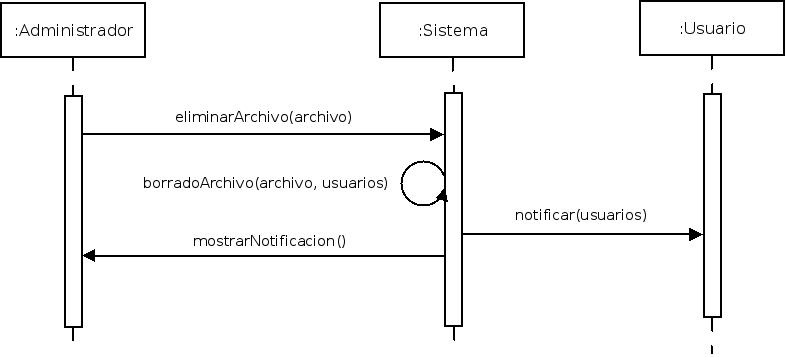
\includegraphics[scale=.50]{img/secuencias/gestion-servicios-eliminar-archivo.jpeg}
  \caption{Diagrama de secuencia: Gestión de servicios: Eliminar archivo}
  \label{fig:secuencia-gestion-servicios-eliminar-archivo}
\end{figure}

\textbf{Contrato de operación: eliminarArchivo(archivo)}
\begin{itemize}
\item \textbf{Referencias cruzadas:} UC-40 (Cuadro \ref{tab:CU-eliminar-archivo}).
\item \textbf{Responsabilidades:} Solicitar al sistema la eliminación del archivo seleccionado.
\item \textbf{Precondiciones:} 
 \begin{itemize}
\item El administrador se ha identificado en el sistema previamente.
\item Existen documentos subidos.
\end {itemize}
\item \textbf{Postcondiciones:} 
 \begin{itemize}
\item El usuario manda al sistema la solicitud de eliminación de un archivo específico.
\end {itemize}
\end {itemize}

\textbf{Contrato de operación: borradoArchivo(archivo)}
\begin{itemize}
\item \textbf{Referencias cruzadas:} UC-40 (Cuadro \ref{tab:CU-eliminar-archivo}).
\item \textbf{Responsabilidades:} Realizar la eliminación del documento seleccionado.
\item \textbf{Precondiciones:} 
 \begin{itemize}
\item El administrador ha solicitado la eliminación de un archivo específico.
\end {itemize}
\item \textbf{Postcondiciones:} 
 \begin{itemize}
\item Los datos del documento seleccionado se eliminarán de la base de datos y el propio archivo de donde esté almacenado.
\end {itemize}
\end {itemize}

\textbf{Contrato de operación: notificar(usuarios)}
\begin{itemize}
\item \textbf{Referencias cruzadas:} UC-40 (Cuadro \ref{tab:CU-eliminar-archivo}).
\item \textbf{Responsabilidades:} Mandar una notificación de documento eliminado a los usuarios con permisos para ver el archivo, en caso que existan.
\item \textbf{Precondiciones:} 
 \begin{itemize}
\item Se ha eliminado del sistema un documento.
\end {itemize}
\item \textbf{Postcondiciones:} 
 \begin{itemize}
\item Se creará una nueva notificación de archivo eliminado para cada uno de los usuarios con permisos de acceso al archivo, especificados por el administrador.
\end {itemize}
\end {itemize}

\textbf{Contrato de operación: mostrarNotificacion()}
\begin{itemize}
\item \textbf{Referencias cruzadas:} UC-40 (Cuadro \ref{tab:CU-eliminar-archivo}).
\item \textbf{Responsabilidades:} Se mostrará un mensaje de acción por pantalla.
\item \textbf{Precondiciones:} 
 \begin{itemize}
\item Se ha realizado la acción correspondiente para activar el mensaje.
\end {itemize}
\item \textbf{Postcondiciones:} 
 \begin{itemize}
\item Se muestra el mensaje correspondiente a la acción en la pantalla, a modo de notificación para el administrador. Este puede ser confirmación de la acción o algún tipo de error en la ejecución de la misma.
\end {itemize}
\end {itemize}


